\documentclass[11pt,a4paper]{article}

% -----------------------------------------------------------------------------
% Configuración
% -----------------------------------------------------------------------------
\usepackage[a4paper,margin=2.5cm]{geometry}
\usepackage[utf8]{inputenc}
\usepackage[T1]{fontenc}
\usepackage{lmodern}
\usepackage[spanish,es-tabla]{babel}
\usepackage{amsmath,amssymb}
\usepackage{graphicx}
\usepackage{float}
\usepackage{booktabs}
\usepackage{array}
\usepackage{longtable}
\usepackage{pdflscape}
\usepackage{listings}
\usepackage[dvipsnames]{xcolor}
\usepackage{caption}
\usepackage{subcaption}
\usepackage{enumitem}
\usepackage{microtype}
\usepackage{algorithm}
\usepackage{algpseudocode}
\usepackage{tikz}
\usetikzlibrary{arrows.meta,positioning,calc,fit}
\usepackage{hyperref}
\usepackage{needspace}

\hypersetup{
    colorlinks=true,
    linkcolor=MidnightBlue,
    citecolor=MidnightBlue,
    urlcolor=MidnightBlue,
    pdftitle={Recuperación de fase con iluminación codificada y HIO},
    pdfauthor={Francisco Alfaro Medina}
}

\setlength{\parindent}{0pt}
\setlength{\parskip}{0.65em}
\setlength{\emergencystretch}{3em}
\renewcommand{\arraystretch}{1.15}
\captionsetup{font=small,labelfont=bf}

\definecolor{codebg}{RGB}{247,248,250}
\definecolor{codecomment}{RGB}{40,120,65}
\lstset{
    language=Python,
    backgroundcolor=\color{codebg},
    basicstyle=\ttfamily\scriptsize,
    keywordstyle=\color{MidnightBlue},
    commentstyle=\color{codecomment},
    stringstyle=\color{BrickRed},
    frame=single,
    rulecolor=\color{gray!45},
    breaklines=true,
    showstringspaces=false,
    columns=fullflexible,
    literate={á}{{\'a}}1 {é}{{\'e}}1 {í}{{\'i}}1 {ó}{{\'o}}1 {ú}{{\'u}}1 {ñ}{{\~n}}1
             {Δ}{{$\Delta$}}1 {β}{{$\beta$}}1 {ψ}{{$\psi$}}1 {⊙}{{$\odot$}}1 {Σ}{{$\Sigma$}}1
             {√}{{$\surd$}}1 {∠}{{$\angle$}}1 {·}{{$\cdot$}}1
}

\algrenewcommand\algorithmicrequire{\textbf{Entrada:}}
\algrenewcommand\algorithmicensure{\textbf{Salida:}}
\floatname{algorithm}{Algoritmo}

\newcommand{\Prop}{\mathcal{P}[\Delta z]}
\newcommand{\PropInv}{\mathcal{P}[-\Delta z]}
\newcommand{\Obj}{\mathbf{O}}
\newcommand{\hio}{\textsc{HIO}}
\newcommand{\er}{\textsc{ER}}
\newcommand{\hioer}{\textsc{HIO/ER}}

\title{
    
\includegraphics[width=5.7cm]{Fig/usm.png}\\[0.35cm]
    \large Universidad Técnica Federico Santa María\\
    Departamento de Informática\\[0.35cm]
    \rule{\linewidth}{0.5pt}\\[0.25cm]
    \LARGE\textbf{Recuperación de fase con iluminación\\
    codificada y el algoritmo Hybrid Input--Output}\\[-0.05cm]
    \rule{\linewidth}{1.5pt}
}
\author{\large Francisco Alfaro Medina\\
\href{mailto:francisco.alfaro@usm.cl}{francisco.alfaro@usm.cl}}
\date{16 de noviembre de 2026}

\begin{document}
\maketitle
\thispagestyle{empty}

\begin{abstract}
Este informe estudia la recuperación de la amplitud y la fase de un objeto complejo a partir de mediciones de intensidad obtenidas con un sistema de iluminación codificada. El frente de onda se modula con $L$ aperturas binarias aleatorias complementarias por pares, se propaga en campo cercano mediante el método de espectro angular y se registra solo su intensidad. El código MATLAB de referencia se portó a Python y el esquema de reconstrucción original se reemplazó por el algoritmo Hybrid Input--Output (\hio{}) de Fienup, extendido a múltiples máscaras mediante una proyección de consenso. Con ruido gaussiano de $40$ dB, \hio{} puro diverge; alternar bloques de \hio{} y Error Reduction (\er{}) lo estabiliza y además alcanza el nivel final casi el doble de rápido que \er{}. Sobre 24 imágenes en escala de grises de $384\times384$, con $L=4$ se obtienen en promedio $44.10$ dB y SSIM $0.987$ en amplitud y $25.57$ dB y SSIM $0.823$ en fase. Con $L=16$ se alcanzan $51.39$ dB y $0.997$ en amplitud y $29.10$ dB y $0.904$ en fase. La mejora se observa en las 24 imágenes y en las cuatro métricas, y $L=16$ converge en 15 iteraciones frente a 25. La principal limitación restante, el error de fase en zonas de amplitud casi nula, no depende de $L$.
\end{abstract}

\tableofcontents
\newpage

\section{Objetivos y alcance}

El objetivo es simular un sistema de iluminación codificada que permita recuperar la amplitud y la fase de un objeto usando aperturas codificadas complementarias. Las actividades realizadas siguen el enunciado de la tarea:

\begin{enumerate}[label=\arabic*.]
    \item portar a Python el código MATLAB del repositorio \texttt{phaseRetrieval-lab} (modelo directo, máscaras y propagador);
    \item generar máscaras aleatorias complementarias por pares para $L=4$ y $L=16$;
    \item reconstruir el objeto con el algoritmo Hybrid Input--Output (\hio{});
    \item usar las 24 imágenes del dataset en escala de grises como amplitud y como fase;
    \item evaluar la calidad espacial con PSNR y SSIM;
    \item graficar las métricas para las 24 imágenes y comparar ambas configuraciones.
\end{enumerate}

El análisis se basa en el notebook \texttt{tareas/tarea-06/homework6.ipynb}, que es ejecutable de principio a fin sin MATLAB ni los archivos \texttt{.mat} del repositorio. Las máscaras, las mediciones y el ruido se generan en Python con semillas fijas, de modo que todas las cifras de este informe son reproducibles.

\section{Fundamento matemático}

\subsection{Importancia de la fase}

En muchos sistemas ópticos el sensor solo registra intensidad, es decir, el módulo al cuadrado del campo complejo. Sin embargo, la mayor parte de la información estructural de una imagen está en la fase de su espectro \cite{oppenheim1981importance}. La Figura~\ref{fig:phase-swap} reproduce, con imágenes del dataset, el experimento de la Fig.~1 del enunciado. Al combinar la magnitud de Fourier de una imagen con la fase de otra, el resultado se parece a la imagen que aporta la fase. Recuperar la fase perdida en la medición es, por lo tanto, esencial para reconstruir el objeto.

\begin{figure}[H]
    \centering
    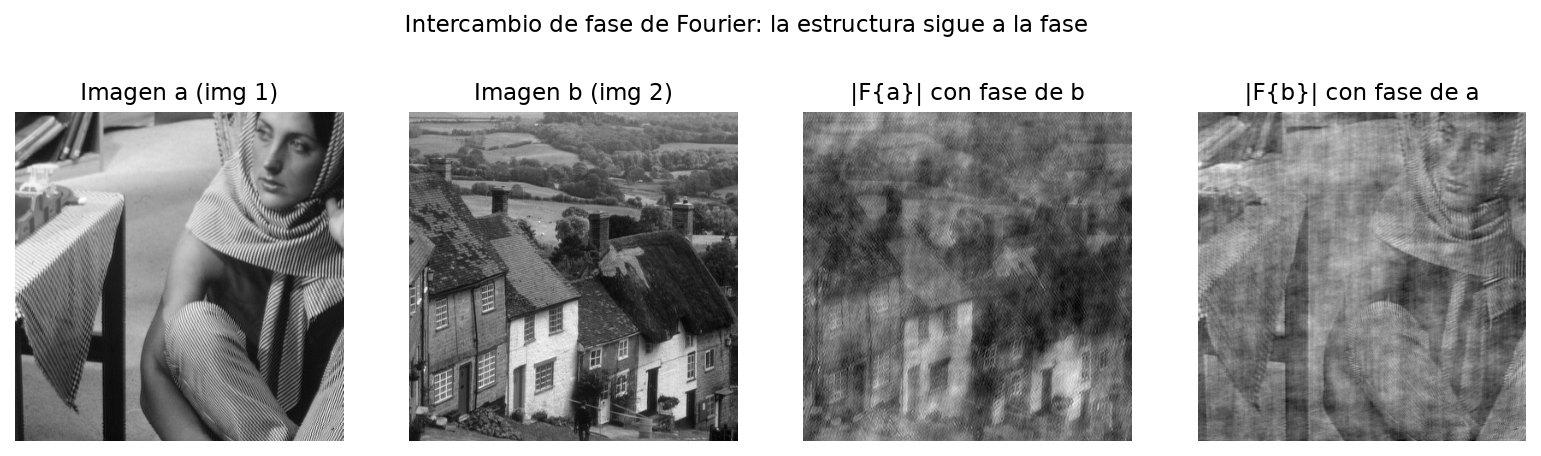
\includegraphics[width=\linewidth]{Fig/phase_swap.png}
    \caption{Intercambio de fase de Fourier entre las imágenes 1 y 2 del dataset. Cada reconstrucción conserva la estructura de la imagen que aporta la fase.}
    \label{fig:phase-swap}
\end{figure}

\subsection{Modelo directo de iluminación codificada}

Un haz coherente y colimado ilumina el objeto y produce un frente de onda complejo desconocido
\begin{equation}
    \Obj = \mathbf{a}\odot e^{i\boldsymbol{\phi}}\in\mathbb{C}^{d\times d},
    \label{eq:objeto}
\end{equation}
donde $\mathbf{a}$ es la amplitud y $\boldsymbol{\phi}$ la fase. El frente de onda se modula con una apertura codificada $\mathbf{A}_\ell\in\{0,1\}^{d\times d}$, $\ell=1,\dots,L$, se propaga una distancia $\Delta z$ y produce un patrón de difracción
\begin{equation}
    \mathbf{I}_\ell=\Prop\{\mathbf{A}_\ell\odot\Obj\}.
    \label{eq:forward}
\end{equation}
El sensor registra
\begin{equation}
    \mathbf{Y}_\ell=|\mathbf{I}_\ell|^2+\boldsymbol{\Omega}_\ell,\qquad \boldsymbol{\Omega}_\ell\in\mathbb{R}^{d\times d},
    \label{eq:medicion}
\end{equation}
donde $|\cdot|$ es el módulo elemento a elemento y $\boldsymbol{\Omega}_\ell$ es ruido aditivo real. La Figura~\ref{fig:diagrama-forward} resume la cadena de adquisición.

\begin{figure}[H]
\centering
\begin{tikzpicture}[
    node distance=0.55cm and 0.75cm,
    blk/.style={draw=MidnightBlue!70, fill=MidnightBlue!6, rounded corners=2pt, minimum height=0.95cm, align=center, font=\small},
    arr/.style={-{Stealth[length=2.2mm]}, thick, MidnightBlue!80}]
    \node[blk] (o) {Objeto\\$\Obj=\mathbf{a}\odot e^{i\boldsymbol\phi}$};
    \node[blk, right=of o] (m) {Apertura\\$\mathbf{A}_\ell\odot\Obj$};
    \node[blk, right=of m] (p) {Propagación\\$\Prop\{\cdot\}$};
    \node[blk, right=of p] (s) {Sensor\\$|\cdot|^2+\boldsymbol\Omega_\ell$};
    \node[blk, right=of s] (y) {Medición\\$\mathbf{Y}_\ell$};
    \draw[arr] (o) -- (m); \draw[arr] (m) -- (p); \draw[arr] (p) -- (s); \draw[arr] (s) -- (y);
    \node[font=\scriptsize, below=0.15cm of m] {$\ell=1,\dots,L$};
\end{tikzpicture}
\caption{Cadena de adquisición: el objeto complejo se modula con cada apertura, se propaga en campo cercano y el sensor registra solo la intensidad.}
\label{fig:diagrama-forward}
\end{figure}

\subsection{Propagador de campo cercano por espectro angular}

El operador $\Prop$ corresponde a la convolución de Fresnel
\begin{equation}
    \mathbf{U}(u,v)=\left[\frac{e^{ik\Delta z}}{i\lambda\Delta z}\,e^{i\frac{k}{2\Delta z}(u^2+v^2)}\right]\otimes\mathbf{U}_0,
    \qquad k=\frac{2\pi}{\lambda},
    \label{eq:fresnel}
\end{equation}
donde $\mathbf{U}_0$ es el campo en el plano fuente y $\mathbf{U}$ el campo en el plano de observación \cite{goodman2005}. Por el teorema de convolución, en el dominio de frecuencias espaciales esta operación es un producto por una función de transferencia cuadrática. La implementación del repositorio sigue el método de espectro angular por pasos de Schmidt \cite{schmidt2010}. Con las DFT centradas
\begin{equation}
    \operatorname{ft2}(g,\delta)=\operatorname{fftshift}\big(\operatorname{fft2}(\operatorname{fftshift}(g))\big)\,\delta^2,
    \qquad
    \operatorname{ift2}(G,\delta f)=\operatorname{ifftshift}\big(\operatorname{ifft2}(\operatorname{ifftshift}(G))\big)\,(N\delta f)^2,
\end{equation}
cada paso entre planos $z_i\to z_{i+1}$ aplica
\begin{equation}
    U\leftarrow\operatorname{ift2}\!\left(Q_2^{(i)}\cdot\operatorname{ft2}\!\left(\frac{U}{m_i},\delta_i\right),\delta f_i\right),
    \qquad
    Q_2^{(i)}=\exp\!\left(i\pi^2\frac{2\Delta z_i}{m_i k}\,(f_x^2+f_y^2)\right),
    \label{eq:q2}
\end{equation}
donde $\delta_i$ es el tamaño de píxel en el plano $i$, $m_i=\delta_{i+1}/\delta_i$ es el factor de escala y $\delta f_i=1/(N\delta_i)$. Los factores cuadráticos de entrada y salida $Q_1$ y $Q_3$ solo intervienen cuando $\delta_1\neq\delta_n$. En este trabajo se usan los parámetros de \texttt{main.m}, $\delta_1=\delta_n$, por lo que $m_i=1$ y $Q_2^{(i)}=\exp(i\pi\lambda\Delta z_i f^2)$.

\paragraph{Implementación eficiente y exacta.} En \hio{} el propagador se evalúa $2L$ veces por iteración. Dos observaciones permiten precalcularlo sin aproximar. Primero, entre pasos consecutivos la pareja $\operatorname{ift2}(\cdot,\delta f_i)$, $\operatorname{ft2}(\cdot,\delta_{i+1})$ se cancela salvo un escalar, de modo que los cuatro pasos se combinan en una sola función de transferencia $H=\prod_i Q_2^{(i)}$ con factor $\prod_i 1/m_i$. Segundo, para $N$ par los \texttt{fftshift} alrededor de un operador de convolución circular se cancelan. Así,
\begin{equation}
    \Prop\{U\}=Q_3\,\mathcal{F}^{-1}\big\{H\cdot\mathcal{F}\{Q_1U\}\big\},
    \label{eq:prop-rapido}
\end{equation}
con 2 FFT en lugar de 8. Igual que en \texttt{PhaseLiftSimu.m}, la retropropagación se obtiene con $-z$. Como $|H|=1$, el operador es unitario y $\PropInv=\Prop^{-1}=\Prop^{H}$.

\paragraph{Criterio de muestreo.} La función de transferencia está bien muestreada (sin aliasing de la fase cuadrática) si
\begin{equation}
    N\geq\frac{\lambda\Delta z}{\delta^2}.
    \label{eq:muestreo}
\end{equation}
Con los parámetros de la Tabla~\ref{tab:parametros}, $\lambda\Delta z/\delta^2=643\cdot10^{-6}\cdot160/0.02^2\approx257.2$. Por eso se eligió $N=384$, el mismo tamaño de \texttt{main.m}. Un tamaño de $256$ habría violado levemente el criterio con los parámetros originales.

\subsection{Aperturas codificadas complementarias}

Siguiendo \texttt{selectMasks.m} y \texttt{complementary\_masks.m}, se generan máscaras binarias i.i.d. con $P(\mathbf{A}=1)=0.5$ y cada máscara par se define como el complemento de la anterior:
\begin{equation}
    \mathbf{A}_{2c}=\mathbf{1}-\mathbf{A}_{2c-1},\qquad c=1,\dots,L/2.
    \label{eq:complementarias}
\end{equation}
Cada par cubre todo el plano, por lo que
\begin{equation}
    \sum_{\ell=1}^{L}\mathbf{A}_\ell=\frac{L}{2}\,\mathbf{1}:
    \label{eq:cobertura}
\end{equation}
cada píxel del objeto se observa exactamente en $L/2$ mediciones (2 con $L=4$ y 8 con $L=16$). Esta propiedad es clave para la restricción de objeto de \hio{} (Sección~\ref{sec:hio}).

\begin{figure}[H]
    \centering
    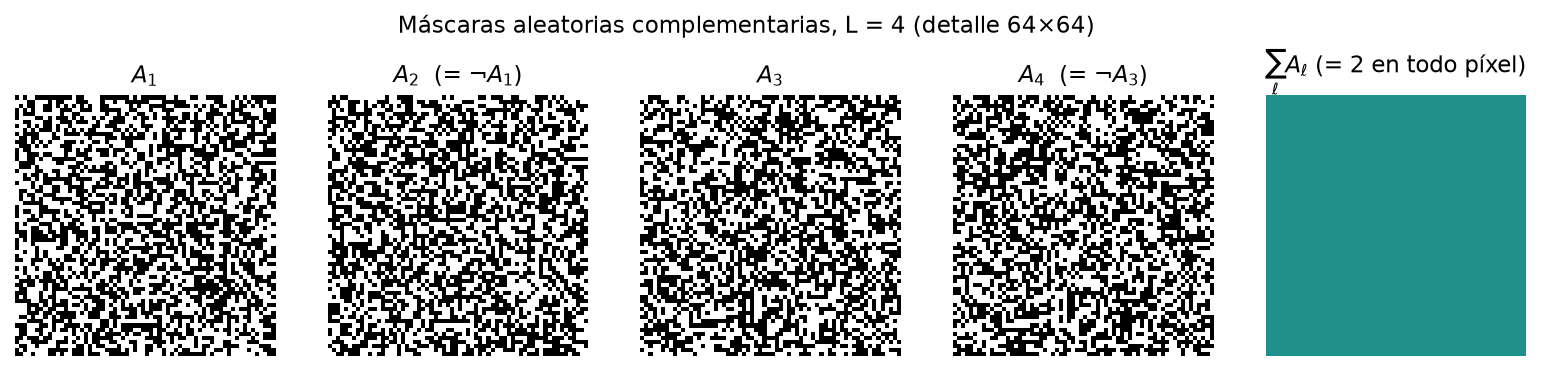
\includegraphics[width=\linewidth]{Fig/masks_L4.png}
    \caption{Máscaras aleatorias complementarias para $L=4$ (detalle $64\times64$). La suma de las cuatro máscaras vale 2 en todos los píxeles.}
    \label{fig:mascaras}
\end{figure}

\paragraph{Número de condición.} La función \texttt{ComputeConditionNumber.m} calcula $\kappa(\mathbf{K}^{\mathsf T}\mathbf{K})$, donde $\mathbf{K}\in\{0,1\}^{d^2\times L}$ tiene las máscaras vectorizadas como columnas. Con pares complementarios se cumple $\mathbf{A}_1+\mathbf{A}_2-\mathbf{A}_3-\mathbf{A}_4=\mathbf{0}$ (y relaciones análogas), así que $\operatorname{rango}(\mathbf{K}^{\mathsf T}\mathbf{K})=L/2+1$ y el número de condición es infinito en la práctica: el notebook obtiene $1.9\times10^{17}$ y $1.7\times10^{18}$, que corresponden al límite de precisión. Esa medida lineal no describe el condicionamiento del problema de recuperación de fase, que es cuadrático en $\Obj$.

\subsection{Problema inverso y ambigüedades}

Recuperar $\Obj$ equivale a resolver
\begin{equation}
    \min_{\Obj}\ f(\Obj)=\sum_{\ell=1}^{L}\big\|\mathbf{Y}_\ell-\mathcal{A}_\ell(\Obj\Obj^{H})\big\|_2^2,
    \label{eq:inverso}
\end{equation}
donde $\mathcal{A}_\ell$ es el operador lineal que lleva $\Obj\Obj^H$ a $|\Prop\{\mathbf{A}_\ell\odot\Obj\}|^2$. Las mediciones son invariantes a una fase global: $\Obj$ y $\Obj e^{i\theta}$ producen exactamente los mismos $\mathbf{Y}_\ell$. La diversidad introducida por las máscaras elimina en general las demás ambigüedades \cite{candes2015coded}, de modo que la solución es única salvo esa constante. Por eso, antes de evaluar, se alinea la fase global (Sección~\ref{sec:alineacion}).

\subsection{Algoritmo Hybrid Input--Output}
\label{sec:hio}

\paragraph{\hio{} clásico.} El algoritmo de Fienup \cite{fienup1982} alterna entre el dominio de medición y el dominio del objeto. Dada la estimación $g_k$:
\begin{enumerate}[label=\arabic*.]
    \item \textbf{Restricción de medición} ($P_M$): $G_k=\Prop\{g_k\}$, $G'_k=\sqrt{\mathbf{Y}}\,e^{i\angle G_k}$ y $g'_k=\PropInv\{G'_k\}$. Se reemplaza la magnitud por la medida y se conserva la fase estimada.
    \item \textbf{Restricción de objeto}: sea $\gamma$ la región donde $g'_k$ satisface las restricciones (soporte, no negatividad, etc.). Entonces
    \begin{equation}
        g_{k+1}(x)=\begin{cases}
            g'_k(x), & x\in\gamma,\\
            g_k(x)-\beta\,g'_k(x), & x\notin\gamma.
        \end{cases}
        \label{eq:hio-clasico}
    \end{equation}
\end{enumerate}
Con $g_{k+1}=g'_k$ en $\gamma$ y $g_{k+1}=0$ fuera de $\gamma$ se obtiene Error Reduction (\er{}), equivalente al algoritmo de Gerchberg--Saxton \cite{gerchberg1972}. Ese es el esquema que implementa \texttt{PhaseLiftSimu.m}. El término $-\beta g'_k$ es la realimentación que permite a \hio{} escapar de los estancamientos de \er{}.

\paragraph{Extensión a $L$ aperturas codificadas.} En el sistema codificado, la restricción de objeto se aplica a las ondas de salida $\boldsymbol\psi_\ell=\mathbf{A}_\ell\odot\Obj$. Para cada máscara, el soporte es $\{x:\mathbf{A}_\ell(x)=1\}$ y, además, las $L$ ondas deben provenir del mismo objeto. El conjunto de restricciones es
\begin{equation}
    \mathcal{S}=\big\{(\boldsymbol\psi_1,\dots,\boldsymbol\psi_L):\ \boldsymbol\psi_\ell=\mathbf{A}_\ell\odot\Obj\ \text{para algún}\ \Obj\big\},
\end{equation}
y su proyección ortogonal se obtiene por mínimos cuadrados:
\begin{equation}
    \widehat{\Obj}=\frac{\sum_\ell\mathbf{A}_\ell\odot\boldsymbol\psi_\ell}{\sum_\ell\mathbf{A}_\ell},
    \qquad
    P_\mathcal{S}(\boldsymbol\psi)_\ell=\mathbf{A}_\ell\odot\widehat{\Obj}.
    \label{eq:ps}
\end{equation}
Por la ecuación~\eqref{eq:cobertura}, el denominador vale $L/2>0$ en todo píxel; las máscaras complementarias garantizan que la proyección esté siempre bien definida. Como $P_\mathcal{S}$ es lineal, \hio{} se escribe en forma compacta \cite{bauschke2002}:
\begin{equation}
    \boxed{\,g_{k+1}=P_\mathcal{S}(g'_k)+(I-P_\mathcal{S})\,(g_k-\beta\,g'_k),\qquad g'_k=P_M(g_k).\,}
    \label{eq:hio-general}
\end{equation}
La componente de $g'_k$ en $\mathcal{S}$ corresponde a la región válida: está en el soporte de $\mathbf{A}_\ell$ y es consistente entre máscaras. La componente $(I-P_\mathcal{S})g'_k$ es la parte que viola las restricciones. Para $L=1$ y una proyección de soporte, la ecuación~\eqref{eq:hio-general} coincide exactamente con~\eqref{eq:hio-clasico}. La Figura~\ref{fig:diagrama-hio} esquematiza una iteración.

\begin{figure}[H]
\centering
\begin{tikzpicture}[
    node distance=0.6cm and 1.0cm,
    blk/.style={draw=MidnightBlue!70, fill=MidnightBlue!6, rounded corners=2pt, minimum height=1.0cm, minimum width=3.3cm, align=center, font=\small},
    arr/.style={-{Stealth[length=2.2mm]}, thick, MidnightBlue!80},
    lbl/.style={font=\scriptsize, fill=white, inner sep=1pt}]
    \node[blk] (g) {Ondas de salida\\$g_k=(\boldsymbol\psi_1,\dots,\boldsymbol\psi_L)$};
    \node[blk, right=2.3cm of g] (G) {Plano sensor\\$G_k=\Prop\{g_k\}$};
    \node[blk, below=1.0cm of G] (Gp) {Magnitud medida\\$G'_k=\sqrt{\mathbf{Y}}\,e^{i\angle G_k}$};
    \node[blk, below=1.0cm of g] (gp) {Retropropagación\\$g'_k=\PropInv\{G'_k\}$};
    \node[blk, below=1.0cm of gp, minimum width=8.5cm] (upd) {Restricción de objeto: $g_{k+1}=P_\mathcal{S}(g'_k)+(I-P_\mathcal{S})(g_k-\beta g'_k)$\\[1pt]
        {\scriptsize consenso $\widehat\Obj=\sum_\ell\mathbf{A}_\ell\odot g'_{k,\ell}\,/\sum_\ell\mathbf{A}_\ell$ \quad (bloques \er{}: $g_{k+1}=P_\mathcal{S}(g'_k)$)}};
    \draw[arr] (g) -- node[lbl, above]{$\Prop$} (G);
    \draw[arr] (G) -- node[lbl, right]{$P_M$} (Gp);
    \draw[arr] (Gp) -- node[lbl, above]{$\PropInv$} (gp);
    \draw[arr] (gp) -- (upd.north -| gp);
    \draw[arr] (upd.west) -- ++(-0.6,0) |- node[lbl, pos=0.25, left]{$k\leftarrow k+1$} (g.west);
\end{tikzpicture}
\caption{Una iteración de \hio{} con $L$ aperturas codificadas. El paso $P_M$ se aplica en paralelo a las $L$ ondas (FFT en lote).}
\label{fig:diagrama-hio}
\end{figure}

\paragraph{Alternancia \hio{}/\er{}.} Con mediciones ruidosas no existe un objeto que satisfaga simultáneamente todas las restricciones ($\mathcal{M}\cap\mathcal{S}=\emptyset$). En ese caso, el término $(I-P_\mathcal{S})(g_k-\beta g'_k)$ acumula en cada iteración la parte de $g'_k$ que no puede anularse, y el iterado se aleja de la solución. Es un comportamiento conocido de \hio{} y de los métodos de reflexión en problemas inconsistentes \cite{luke2005raar}. Siguiendo la recomendación de Fienup, se alternan bloques de 10 iteraciones \hio{} con bloques de 10 iteraciones \er{} ($g_{k+1}=P_\mathcal{S}(g'_k)$). Cada bloque \er{} devuelve el iterado al conjunto $\mathcal{S}$ y descarta la realimentación acumulada; los bloques \hio{} conservan la capacidad de escapar de estancamientos. La Sección~\ref{sec:ablation} justifica esta elección experimentalmente.

\paragraph{Métrica de convergencia.} Se usa el error de dominio objeto de Fienup,
\begin{equation}
    E_k=\frac{\|(I-P_\mathcal{S})\,g'_k\|_2}{\|g'_k\|_2},
    \label{eq:ek}
\end{equation}
que es la fracción de energía que viola las restricciones. Vale cero en una solución exacta y no requiere conocer el objeto real.

\paragraph{Inicialización.} Igual que en \texttt{main.m} (\texttt{fieldvec = ones(M,N)}), se usa un objeto constante, escalado para que su energía coincida con la medida. Como la propagación es unitaria y las máscaras son binarias, $\sum_\ell\|\mathbf{Y}_\ell\|_1=\sum_\ell\|\mathbf{A}_\ell\odot\Obj\|_2^2$ en ausencia de ruido.

\begin{algorithm}[H]
\caption{\hio{} con $L$ aperturas codificadas y alternancia \hio{}/\er{}.}
\label{alg:hio}
\begin{algorithmic}[1]
\Require Mediciones $\{\mathbf{Y}_\ell\}$, máscaras $\{\mathbf{A}_\ell\}$, $\beta$, $K$ iteraciones, bloques $(n_\text{HIO},n_\text{ER})$
\Ensure Estimación $\widehat\Obj$
\State $w\gets\sum_\ell\mathbf{A}_\ell$; \quad $\Obj_0\gets c\,\mathbf{1}$ con $c^2=\sum_\ell\|\mathbf{Y}_\ell\|_1/\|w\|_1$; \quad $g_{0,\ell}\gets\mathbf{A}_\ell\odot\Obj_0$
\For{$k=0,\dots,K-1$}
    \State $G_\ell\gets\Prop\{g_{k,\ell}\}$ \Comment{para todo $\ell$, en lote}
    \State $g'_\ell\gets\PropInv\big\{\sqrt{\max(\mathbf{Y}_\ell,0)}\;G_\ell/|G_\ell|\big\}$
    \State $\widehat\Obj\gets\sum_\ell\mathbf{A}_\ell\odot g'_\ell\,/\,w$; \quad $p_\ell\gets\mathbf{A}_\ell\odot\widehat\Obj$ \Comment{$P_\mathcal{S}(g')$}
    \State $E_k\gets\|g'-p\|/\|g'\|$
    \If{$k \bmod (n_\text{HIO}+n_\text{ER})<n_\text{HIO}$} \Comment{bloque \hio{}}
        \State $q_\ell\gets\mathbf{A}_\ell\odot\big(\sum_j\mathbf{A}_j\odot g_{k,j}/w\big)$ \Comment{$P_\mathcal{S}(g_k)$}
        \State $g_{k+1,\ell}\gets p_\ell+(g_{k,\ell}-q_\ell)-\beta\,(g'_\ell-p_\ell)$
    \Else \Comment{bloque \er{}}
        \State $g_{k+1,\ell}\gets p_\ell$
    \EndIf
\EndFor
\State \Return $\widehat\Obj$
\end{algorithmic}
\end{algorithm}

\section{Métricas de evaluación}

Las métricas comparan, por separado, la amplitud reconstruida $|\widehat\Obj|$ con la amplitud real $\mathbf{a}$ y la fase reconstruida $\angle\widehat\Obj$ con la fase real $\boldsymbol\phi$. Ambas están en $[0,1]$.

\subsection{MSE y PSNR}

El error cuadrático medio es
\begin{equation}
 \operatorname{MSE}=\frac{1}{m\,n}\sum_{i=0}^{m-1}\sum_{j=0}^{n-1}\big[I(i,j)-K(i,j)\big]^2,
 \label{eq:mse}
\end{equation}
y el PSNR se define como
\begin{equation}
 \operatorname{PSNR}=10\log_{10}\left(\frac{\operatorname{MAX}_I^2}{\operatorname{MSE}}\right),\qquad \operatorname{MAX}_I=1.
 \label{eq:psnr}
\end{equation}
Las imágenes son de tipo flotante en $[0,1]$, de modo que $\operatorname{MAX}_I=1$ equivale a $255$ en 8 bits. En el notebook, la función \texttt{psnr\_eq} implementa literalmente las ecuaciones~\eqref{eq:mse}--\eqref{eq:psnr} y coincide con \texttt{skimage.metrics.peak\_signal\_noise\_ratio} en todos los decimales mostrados ($44.457036$ dB en el caso de prueba).

\subsection{SSIM}

El índice de similitud estructural \cite{wang2004ssim} es
\begin{equation}
 \operatorname{SSIM}(x,y)=
 \frac{(2\mu_x\mu_y+C_1)(2\sigma_{xy}+C_2)}
 {(\mu_x^2+\mu_y^2+C_1)(\sigma_x^2+\sigma_y^2+C_2)},
 \qquad C_1=(K_1L)^2,\ C_2=(K_2L)^2,
 \label{eq:ssim}
\end{equation}
donde $\mu$, $\sigma^2$ y $\sigma_{xy}$ son medias, varianzas y covarianza locales. Igual que la función \texttt{ssim} de MATLAB, las estadísticas locales se calculan con una ventana gaussiana de $\sigma=1.5$ ($11\times11$), con $K_1=0.01$, $K_2=0.03$ y rango dinámico $L=1$; el índice final es el promedio del mapa SSIM sin el borde de la ventana. La implementación propia \texttt{ssim\_eq} coincide con \texttt{skimage.metrics.structural\_similarity} configurada de la misma forma ($0.984973$ en el caso de prueba).

\subsection{Alineación de la fase global}
\label{sec:alineacion}

Como las mediciones no determinan la fase global, antes de evaluar se corrige la reconstrucción:
\begin{equation}
    \widehat\Obj\leftarrow\widehat\Obj\,e^{-i\theta^\star},\qquad
    \theta^\star=\angle\langle\Obj,\widehat\Obj\rangle=\angle\sum_{x}\overline{\Obj(x)}\,\widehat\Obj(x).
    \label{eq:alineacion}
\end{equation}
Después se recortan $|\widehat\Obj|$ y $\angle\widehat\Obj$ al rango $[0,1]$ del valor real. \texttt{main.m} normaliza la reconstrucción con \texttt{mat2gray}; eso también compensa el desfase, pero estira el rango cuando hay valores extremos en zonas oscuras. Se prefirió la alineación~\eqref{eq:alineacion}, que es la práctica estándar en recuperación de fase.

\subsection{Rangos orientativos}

Los umbrales no son universales. Se utiliza la misma guía interpretativa de informes anteriores del curso.

\begin{table}[H]
\centering
\caption{Rangos orientativos para interpretar las métricas.}
\label{tab:rangos}
\begin{tabular}{>{\raggedright\arraybackslash}p{2.2cm}p{2.8cm}p{2.8cm}p{2.8cm}p{2.2cm}}
\toprule
Métrica & Bajo o malo & Intermedio & Bueno & Mejor valor \\
\midrule
PSNR (dB) & $<20$ & $20$--$30$ & $\geq30$ & $\infty$ \\
SSIM & $<0.70$ & $0.70$--$0.85$ & $\geq0.85$ & $1$ \\
\bottomrule
\end{tabular}
\end{table}

\section{Protocolo experimental}

\subsection{Dataset y preprocesamiento}

Se usan las 24 imágenes en escala de grises entregadas con la tarea (\texttt{dataset/1.gif}--\texttt{24.gif}, de $512\times512$). El preprocesamiento replica \texttt{main.m}:

\begin{enumerate}[label=\arabic*.]
    \item convertir a tipo flotante y normalizar a $[0,1]$ con mínimo--máximo (equivalente a \texttt{mat2gray});
    \item recortar la región central de $384\times384$, sin interpolación.
\end{enumerate}

\begin{figure}[H]
    \centering
    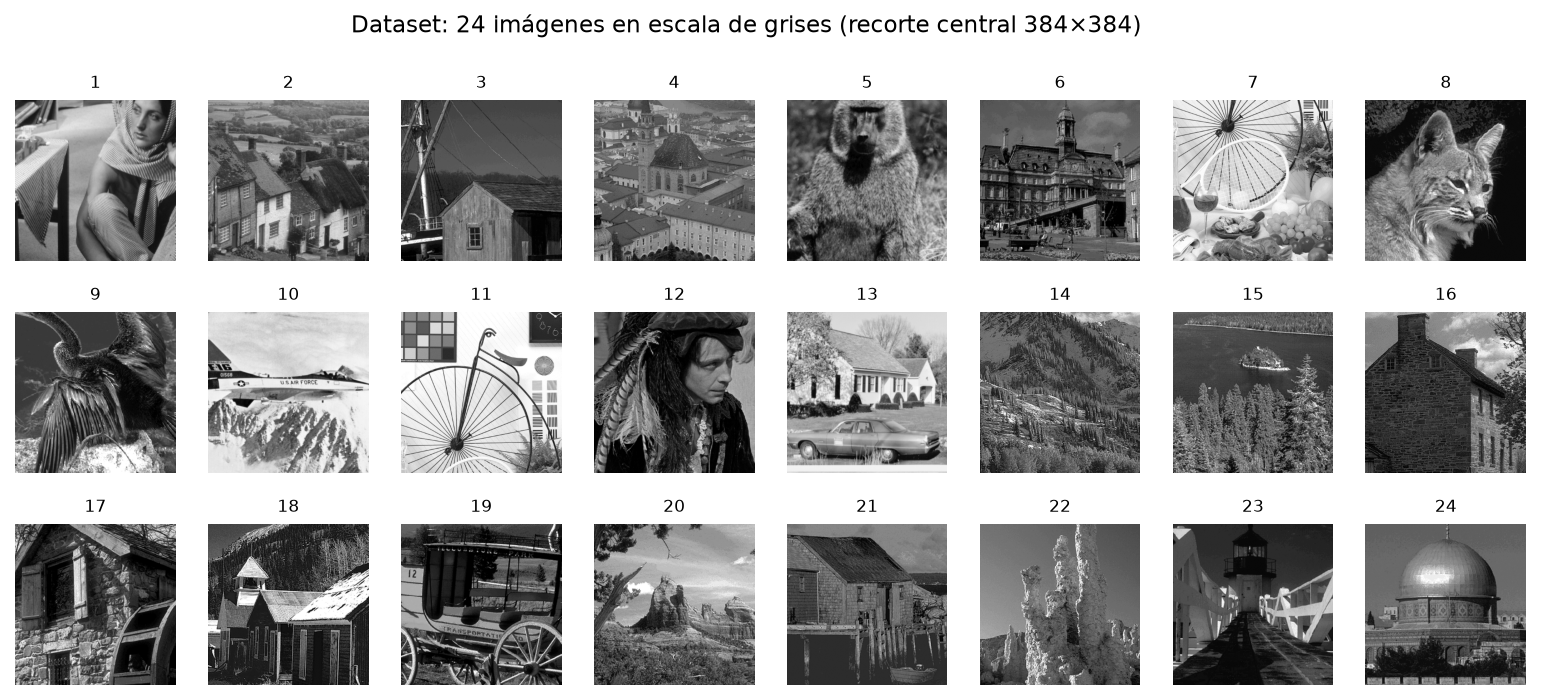
\includegraphics[width=\linewidth]{Fig/dataset.png}
    \caption{Las 24 imágenes del dataset tras el recorte central de $384\times384$.}
    \label{fig:dataset}
\end{figure}

Para cada $k=1,\dots,24$ se construye el objeto
\begin{equation}
    \Obj_k=\mathbf{x}_{25-k}\odot e^{i\,\mathbf{x}_k},
    \label{eq:objeto-k}
\end{equation}
donde $\mathbf{x}_k$ es la imagen $k$. Así, la imagen $k$ actúa como fase y la imagen $25-k$ como amplitud, igual que en \texttt{main.m}, y cada imagen se usa una vez como amplitud y una vez como fase. La fase queda en $[0,1]$ rad, como en el código de referencia, por lo que no hay ambigüedad de \emph{wrapping}.

\subsection{Parámetros}

\begin{table}[H]
\centering
\caption{Parámetros físicos y algorítmicos de los experimentos.}
\label{tab:parametros}
\small
\begin{tabular}{>{\raggedright\arraybackslash}p{4.3cm}>{\raggedright\arraybackslash}p{3.6cm}>{\raggedright\arraybackslash}p{6.2cm}}
\toprule
Parámetro & Valor & Comentario \\
\midrule
Longitud de onda $\lambda$ & $643$ nm & igual que \texttt{main.m} (\texttt{wvl = 643e-6} mm) \\
Píxel DMD / cámara $\delta_1,\delta_n$ & $20\ \mu$m & $\delta_1=\delta_n\Rightarrow Q_1=Q_3=1$ \\
Propagación $\Delta z$ & $160$ mm & 4 pasos de 40 mm (\texttt{linspace(0,160,5)}) \\
Tamaño $N\times N$ & $384\times384$ & cumple $N\geq\lambda\Delta z/\delta^2\approx257$ \\
Máscaras & aleatorias complementarias & $L\in\{4,16\}$, semilla fija por $L$ \\
Ruido $\boldsymbol\Omega$ & gaussiano, SNR $=40$ dB & $\sigma^2=\overline{|\mathbf{I}|^4}/10^{4}$, semilla fija por $(L,k)$ \\
Algoritmo & \hio{}/\er{}, $\beta=0.9$ & bloques de 10 \hio{} + 10 \er{} \\
Iteraciones & $100$ (fijo) & 5 ciclos; terminan en un bloque \er{} \\
\bottomrule
\end{tabular}
\end{table}

\subsection{Procedimiento}

Para cada configuración $L\in\{4,16\}$ y cada objeto $k$:

\begin{enumerate}[label=\arabic*.]
    \item construir $\Obj_k$ según la ecuación~\eqref{eq:objeto-k};
    \item simular las $L$ mediciones $\mathbf{Y}_\ell$ con las ecuaciones~\eqref{eq:forward}--\eqref{eq:medicion};
    \item reconstruir con el Algoritmo~\ref{alg:hio}, registrando $E_k$ y la PSNR por iteración;
    \item alinear la fase global y calcular PSNR y SSIM de la amplitud y de la fase;
    \item reportar resultados por imagen, promedio y desviación estándar.
\end{enumerate}

Ambas configuraciones usan el mismo número de iteraciones, el mismo $\beta$ y el mismo SNR por medición. Se usa un número fijo de iteraciones en lugar de una tolerancia sobre $E_k$ porque, con ruido, $E_k$ no tiende a cero sino a un piso que depende del SNR y de $L$. Como experimento complementario, el mismo protocolo se repite sin ruido.

\subsection{Implementación reproducible}

El núcleo de la implementación es:

\begin{lstlisting}[caption={Propagador precalculado y cuerpo de \texttt{hio\_reconstruct}.},label={lst:hio}]
prop_fwd = NearFieldPropagator(M, WVL, DELTA1, DELTAN, Z)     # P[Δz]
prop_bwd = NearFieldPropagator(M, WVL, DELTA1, DELTAN, -Z)    # P[-Δz]

for it in range(n_iter):
    G = prop_fwd(g)                                    # P[Δz]{ψ_l}, las L ondas en lote
    G_new = sqrtY * G / np.maximum(np.abs(G), 1e-30)   # √Y_l · exp(i∠G_l)
    g_prime = prop_bwd(G_new)                          # g'_k
    O_hat = (A * g_prime).sum(axis=0) / weight         # objeto consenso
    PS_gp = A * O_hat[None]                            # P_S(g'_k)
    violation = g_prime - PS_gp                        # (I - P_S) g'_k
    history[it] = np.linalg.norm(violation) / np.linalg.norm(g_prime)
    if schedule[it]:                                   # bloque HIO
        PS_g = A * ((A * g).sum(axis=0) / weight)[None]
        g = PS_gp + (g - PS_g) - beta * violation
    else:                                              # bloque ER
        g = PS_gp
\end{lstlisting}

La función completa \texttt{hio\_reconstruct(Y\_list, masks, prop\_fwd, prop\_bwd, n\_iter, beta, ...)} retorna la estimación compleja $\widehat\Obj$ y, opcionalmente, el historial de $E_k$. Las semillas son fijas (\texttt{np.random.seed(4)}, igual que \texttt{rng(4)} en \texttt{main.m}, y generadores \texttt{default\_rng} independientes para máscaras y ruido).

\section{Resultados}

\subsection{Verificación del modelo directo}

Antes de reconstruir se verificó numéricamente el propagador (Tabla~\ref{tab:verificacion}). El port coincide con el código MATLAB traducido literalmente, incluso en el caso general $\delta_1\neq\delta_n$; además conserva la energía y su inversa es exacta. La versión precalculada es unas 11 veces más rápida.

\begin{table}[H]
\centering
\caption{Verificaciones numéricas del propagador ($N=384$).}
\label{tab:verificacion}
\small
\begin{tabular}{>{\raggedright\arraybackslash}p{10.6cm}r}
\toprule
Verificación & Resultado \\
\midrule
Error relativo: rápido vs.\ port literal de \texttt{ang\_spec\_multi\_prop} (forward) & $1.8\times10^{-14}$ \\
Error relativo: rápido vs.\ port literal (backward, $-z$) & $1.6\times10^{-14}$ \\
Error relativo: multipaso vs.\ un paso (\texttt{ang\_spec\_pro}) & $9.8\times10^{-16}$ \\
Error relativo: caso general $\delta_1=0.02$, $\delta_n=0.03$ mm & $8.2\times10^{-14}$ \\
Conservación de energía $\|\Prop\{U\}\|/\|U\|$ & $1.000000000000001$ \\
Inversa $\max|\PropInv\Prop\{U\}-U|$ & $1.1\times10^{-15}$ \\
Tiempo para 16 campos: rápido vs.\ literal & $\approx21$ ms vs.\ $\approx229$ ms \\
\bottomrule
\end{tabular}
\end{table}

La Figura~\ref{fig:forward} muestra el modelo directo para el objeto $k=1$. Tras $160$ mm de propagación, el patrón de intensidad ya no se parece al objeto: la información está codificada en la difracción. Las dos mediciones de un par complementario son claramente distintas.

\begin{figure}[H]
    \centering
    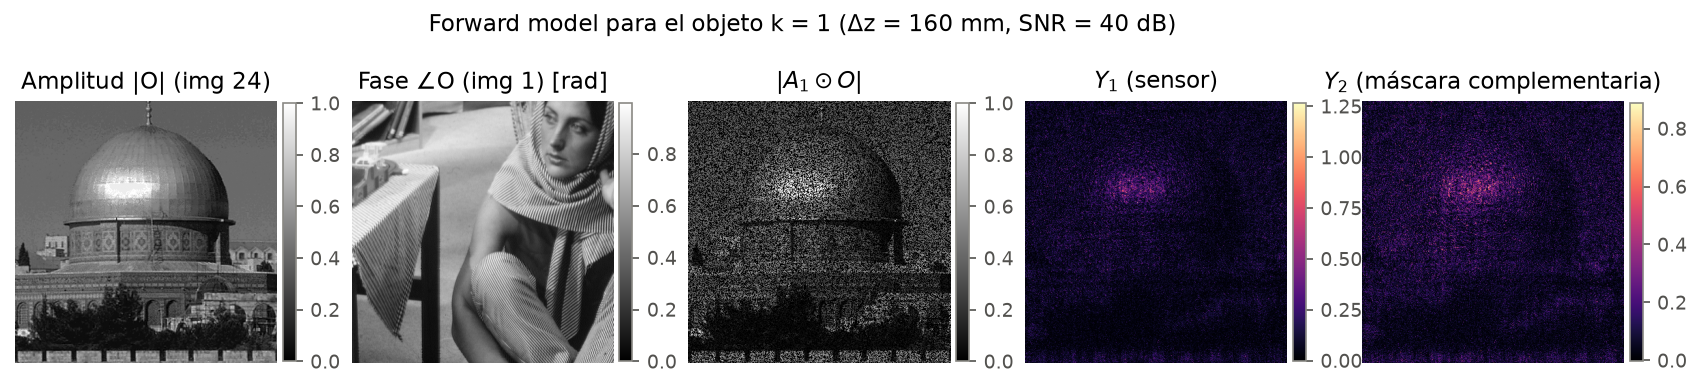
\includegraphics[width=\linewidth]{Fig/forward_example.png}
    \caption{Modelo directo para el objeto $k=1$: amplitud (imagen 24), fase (imagen 1), objeto modulado por $\mathbf{A}_1$ y las mediciones $\mathbf{Y}_1$ y $\mathbf{Y}_2$ de un par complementario.}
    \label{fig:forward}
\end{figure}

\subsection{Selección del esquema y de \texorpdfstring{$\beta$}{beta}}
\label{sec:ablation}

Se compararon cinco variantes con $L=4$, SNR de $40$ dB, 200 iteraciones y los objetos $k=1$, $8$ y $16$ (Figura~\ref{fig:ablation} y Tabla~\ref{tab:ablation}).

\begin{figure}[H]
    \centering
    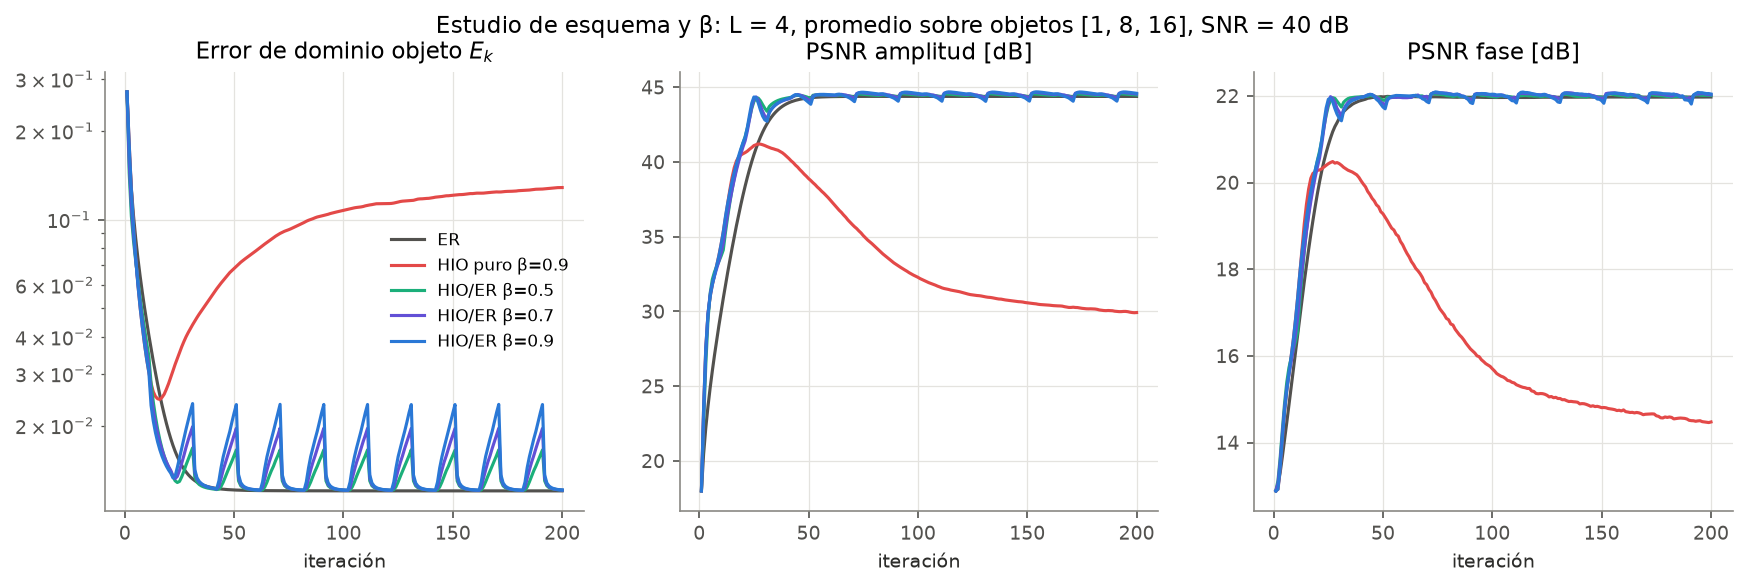
\includegraphics[width=\linewidth]{Fig/beta_ablation.png}
    \caption{Estudio del esquema de reconstrucción: error $E_k$ y PSNR de amplitud y fase por iteración, promedio sobre los objetos 1, 8 y 16 con $L=4$. \hio{} puro (rojo) diverge; las variantes \hio{}/\er{} alcanzan el nivel final antes que \er{}.}
    \label{fig:ablation}
\end{figure}

\begin{table}[H]
\centering
\caption{PSNR media de amplitud y de fase (dB) en las iteraciones 25, 50, 100 y 200, y error $E_k$ final.}
\label{tab:ablation}
\begin{tabular}{lrrrrrrrrr}
\toprule
 & \multicolumn{4}{c}{PSNR amplitud} & \multicolumn{4}{c}{PSNR fase} & \\
\cmidrule(lr){2-5}\cmidrule(lr){6-9}
Variante & 25 & 50 & 100 & 200 & 25 & 50 & 100 & 200 & $E_{200}$ \\
\midrule
\er{} & 40.5 & 44.3 & 44.4 & 44.4 & 20.9 & 22.0 & 22.0 & 22.0 & $1.20\times10^{-2}$ \\
\hio{} puro, $\beta=0.9$ & 41.1 & 38.9 & 32.3 & 29.9 & 20.4 & 19.3 & 15.7 & 14.5 & $1.29\times10^{-1}$ \\
\hio{}/\er{}, $\beta=0.5$ & 44.0 & 44.3 & 44.5 & 44.5 & 21.8 & 21.9 & 22.0 & 22.0 & $1.21\times10^{-2}$ \\
\hio{}/\er{}, $\beta=0.7$ & 44.2 & 44.2 & 44.5 & 44.5 & 21.8 & 21.8 & 22.0 & 22.0 & $1.21\times10^{-2}$ \\
\hio{}/\er{}, $\beta=0.9$ & 44.4 & 44.0 & 44.6 & 44.6 & 21.9 & 21.7 & 22.0 & 22.0 & $1.21\times10^{-2}$ \\
\bottomrule
\end{tabular}
\end{table}

Se observa lo siguiente:
\begin{itemize}
    \item \er{} converge de forma monótona y estable, pero lenta: necesita unas 50 iteraciones para alcanzar $\approx44.4$ dB.
    \item \hio{} puro avanza rápido al comienzo, pero luego \textbf{diverge}: la PSNR de amplitud cae a $29.9$ dB y $E_k$ crece a $0.13$, un orden de magnitud por encima del resto. Es la acumulación de inconsistencia descrita en la Sección~\ref{sec:hio}.
    \item \hio{}/\er{} alcanza $\approx44$ dB ya en la iteración 25, casi el doble de rápido que \er{}, y se mantiene estable. Los picos periódicos de $E_k$ en la Figura~\ref{fig:ablation} corresponden a los bloques \hio{}, donde el iterado sale deliberadamente de $\mathcal{S}$.
    \item El valor de $\beta\in[0.5,0.9]$ influye poco. Se eligió $\beta=0.9$, el valor clásico de Fienup, que entrega la convergencia inicial más rápida.
\end{itemize}

Como la PSNR cambia menos de $0.3$ dB después de la iteración 50, se fijaron 100 iteraciones (5 ciclos \hio{}/\er{}) para los experimentos completos.

\Needspace{14\baselineskip}
\subsection{Resumen estadístico}

La Tabla~\ref{tab:resumen} presenta el promedio y la desviación estándar sobre las 24 imágenes.

\begin{table}[H]
\centering
\caption{Promedio $\pm$ desviación estándar de las métricas sobre las 24 imágenes (SNR $=40$ dB, 100 iteraciones).}
\label{tab:resumen}
\begin{tabular}{lrr}
\toprule
Métrica & $L=4$ & $L=16$ \\
\midrule
PSNR amplitud (dB) & $44.10\pm1.94$ & $51.39\pm1.96$ \\
SSIM amplitud & $0.9870\pm0.0073$ & $0.9974\pm0.0015$ \\
PSNR fase (dB) & $25.57\pm5.75$ & $29.10\pm7.41$ \\
SSIM fase & $0.8231\pm0.0970$ & $0.9038\pm0.0806$ \\
\midrule
Tiempo por imagen (s) & $1.48$ & $5.27$ \\
Tiempo por iteración (ms) & $14.8$ & $52.7$ \\
Iteraciones hasta converger (mediana) & 25 & 15 \\
$E_k$ final (mediana) & $1.11\times10^{-2}$ & $1.47\times10^{-2}$ \\
\bottomrule
\end{tabular}
\end{table}

La diferencia entre configuraciones es
\begin{equation}
 \begin{aligned}
 \Delta\operatorname{PSNR}_\text{amp}&=+7.29\ \mathrm{dB}, &\qquad \Delta\operatorname{SSIM}_\text{amp}&=+0.0104,\\
 \Delta\operatorname{PSNR}_\text{fase}&=+3.53\ \mathrm{dB}, &\qquad \Delta\operatorname{SSIM}_\text{fase}&=+0.0807.
 \end{aligned}
 \label{eq:ganancias}
\end{equation}
En amplitud, la ganancia equivale a reducir el MSE medio unas $5.3$ veces, de $4.3\times10^{-5}$ a $8.1\times10^{-6}$. En fase, el MSE medio baja de $6.4\times10^{-3}$ a $4.4\times10^{-3}$. Todas las reconstrucciones de amplitud quedan en el rango ``bueno'' de la Tabla~\ref{tab:rangos}. La fase queda en promedio en el rango intermedio con $L=4$ y cerca del límite del rango bueno con $L=16$, con gran dispersión entre imágenes.

\subsection{Resultados por imagen}

La Figura~\ref{fig:por-imagen} muestra las cuatro métricas para cada objeto. $L=16$ supera a $L=4$ en las 24 imágenes y en las cuatro métricas. La ganancia de amplitud es notablemente uniforme, entre $+7.21$ y $+7.40$ dB; la de fase varía entre $+0.75$ dB ($k=6$) y $+7.12$ dB ($k=23$). La Figura~\ref{fig:boxplot} resume las distribuciones, y la tabla completa se incluye en el Anexo~\ref{app:tabla-final}.

\begin{figure}[H]
    \centering
    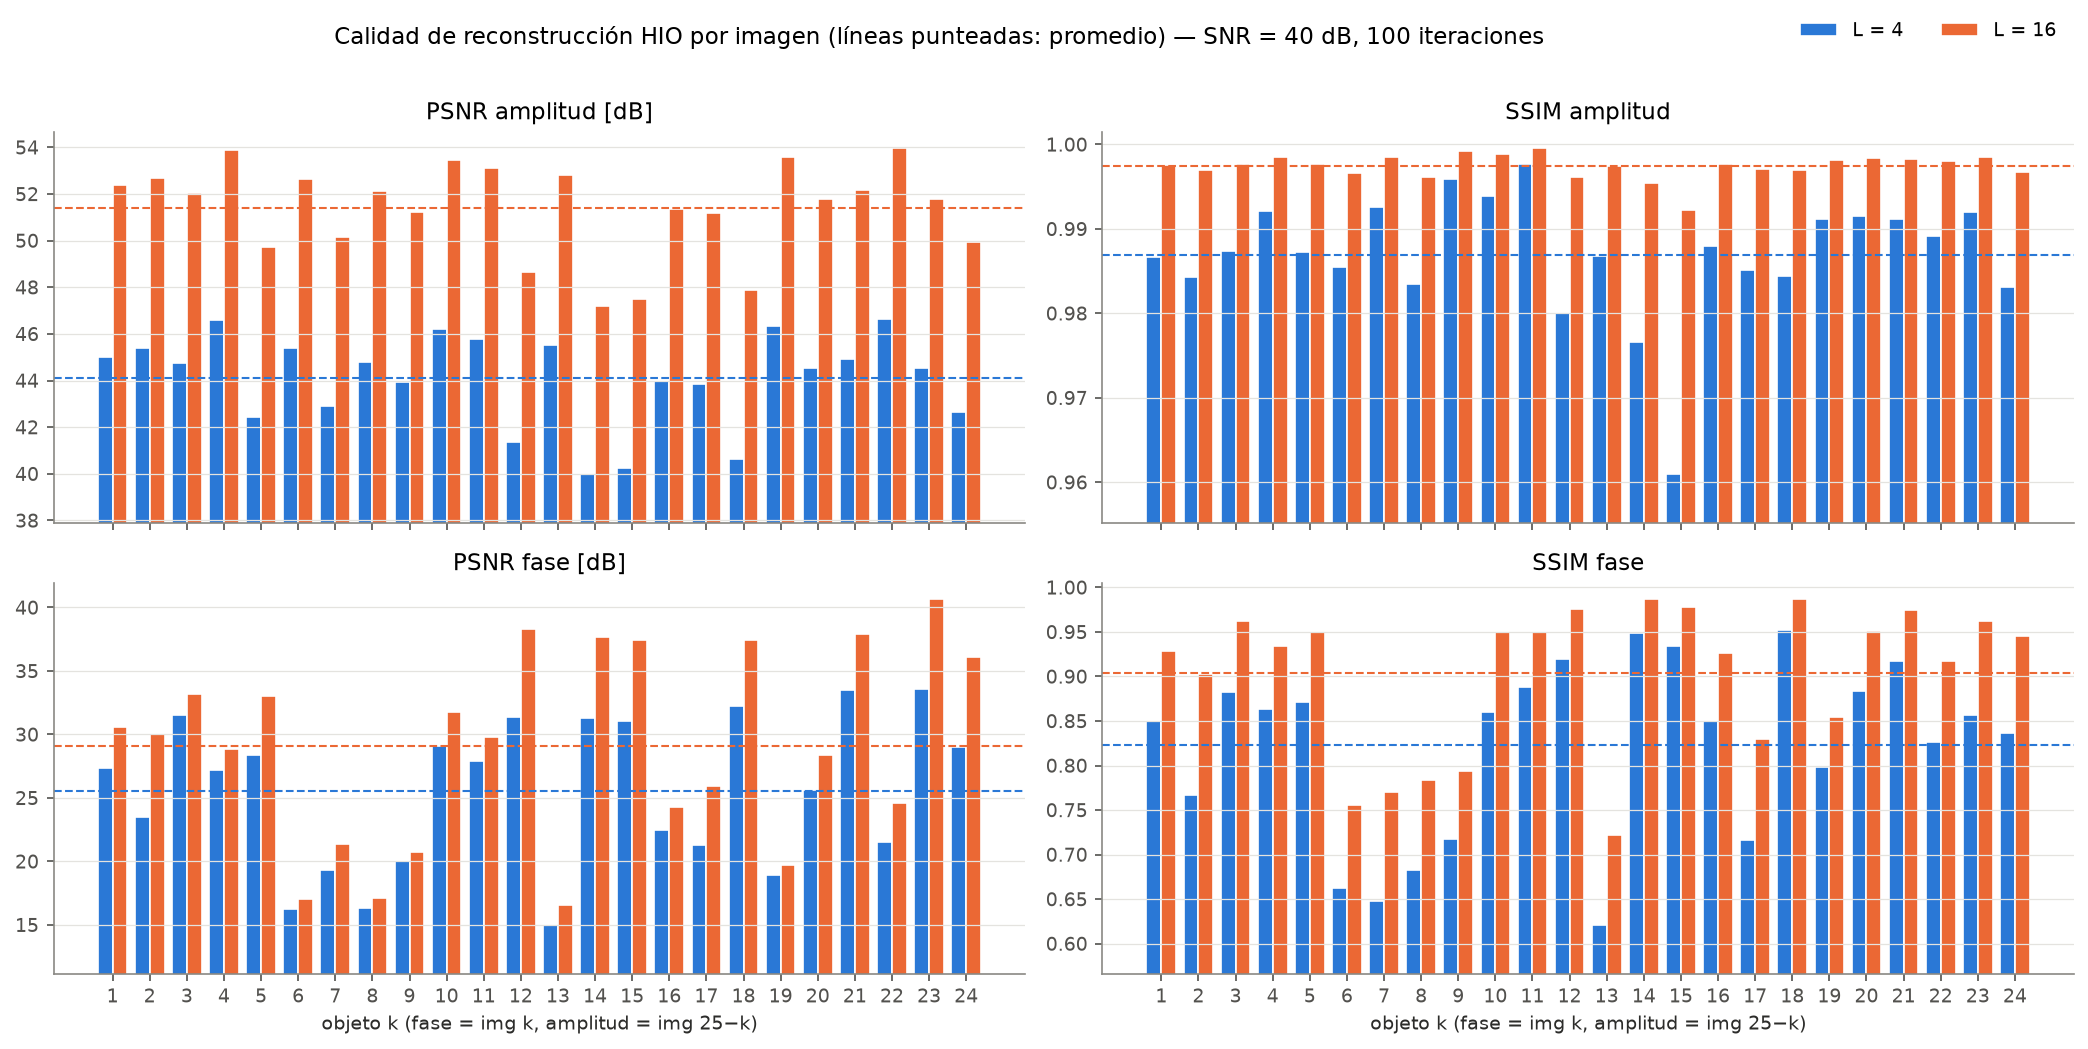
\includegraphics[width=\linewidth]{Fig/metrics_per_image.png}
    \caption{PSNR y SSIM de amplitud y fase por objeto $k$ (fase = imagen $k$, amplitud = imagen $25-k$). Las líneas punteadas indican el promedio de cada configuración.}
    \label{fig:por-imagen}
\end{figure}

\begin{figure}[H]
    \centering
    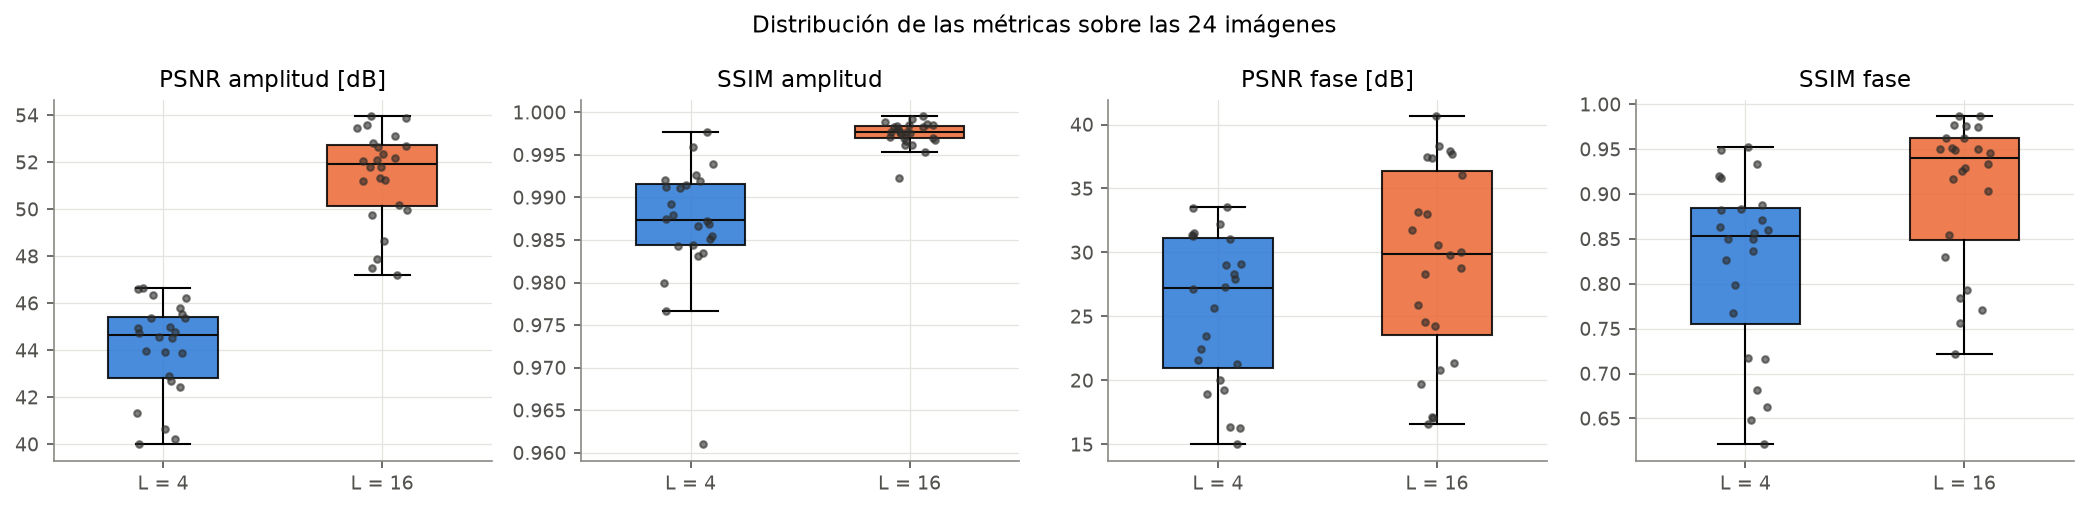
\includegraphics[width=\linewidth]{Fig/metrics_boxplot.png}
    \caption{Distribución de las métricas sobre las 24 imágenes. Cada punto es un objeto.}
    \label{fig:boxplot}
\end{figure}

\subsection{Convergencia}

La Figura~\ref{fig:convergencia} muestra la mediana y la banda entre los percentiles 10 y 90 de $E_k$ y de la PSNR por iteración. Con $L=16$, la PSNR queda a menos de $0.5$ dB de su valor final en una mediana de 15 iteraciones (máximo 16), frente a 25 con $L=4$; para la fase, la mediana es de 12 frente a 24 iteraciones. Las franjas grises marcan los bloques \er{}: durante los bloques \hio{} la PSNR baja levemente y $E_k$ sube, y cada bloque \er{} recupera el nivel. Por eso conviene que la ejecución termine en un bloque \er{}.

\begin{figure}[H]
    \centering
    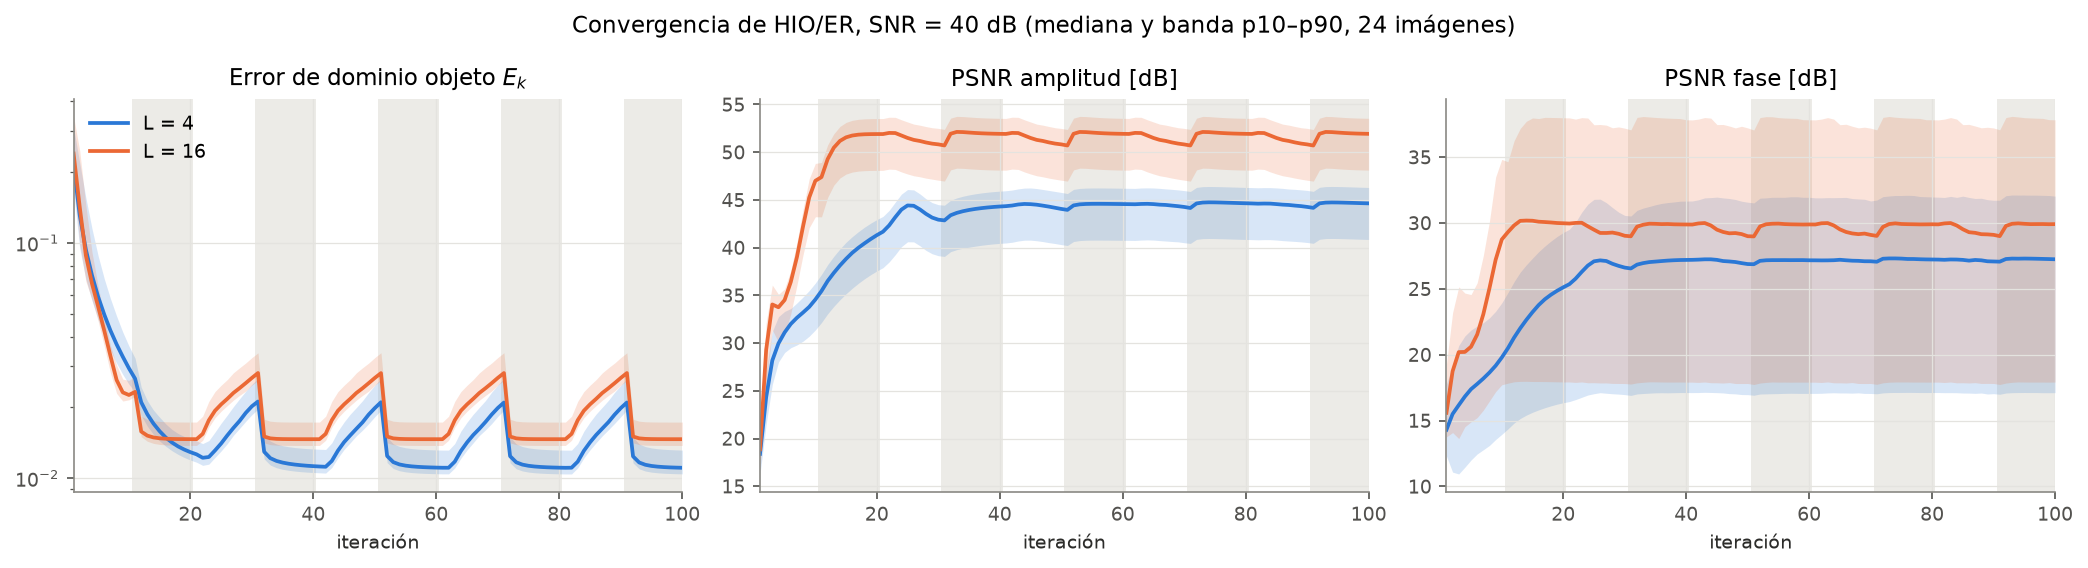
\includegraphics[width=\linewidth]{Fig/convergence.png}
    \caption{Convergencia de \hio{}/\er{} con SNR de $40$ dB: mediana (línea) y banda p10--p90 sobre las 24 imágenes. Las franjas grises son los bloques \er{}.}
    \label{fig:convergencia}
\end{figure}

\subsection{Comparación visual}

La Figura~\ref{fig:visual} muestra tres objetos: el de mejor PSNR de fase con $L=4$ ($k=23$), uno intermedio ($k=1$) y el peor ($k=13$). Las amplitudes son prácticamente indistinguibles del valor real en los tres casos. En la fase, el error se concentra en regiones específicas: en $k=1$, en la vegetación oscura de la parte inferior, y en $k=13$, en la ropa y el fondo oscuros. Esas regiones coinciden con las zonas oscuras de la imagen de amplitud, no de la imagen de fase. $L=16$ reduce la extensión y la intensidad de esos errores, pero no los elimina. Las 24 reconstrucciones se incluyen en el Anexo~\ref{app:visual}.

\begin{figure}[H]
    \centering
    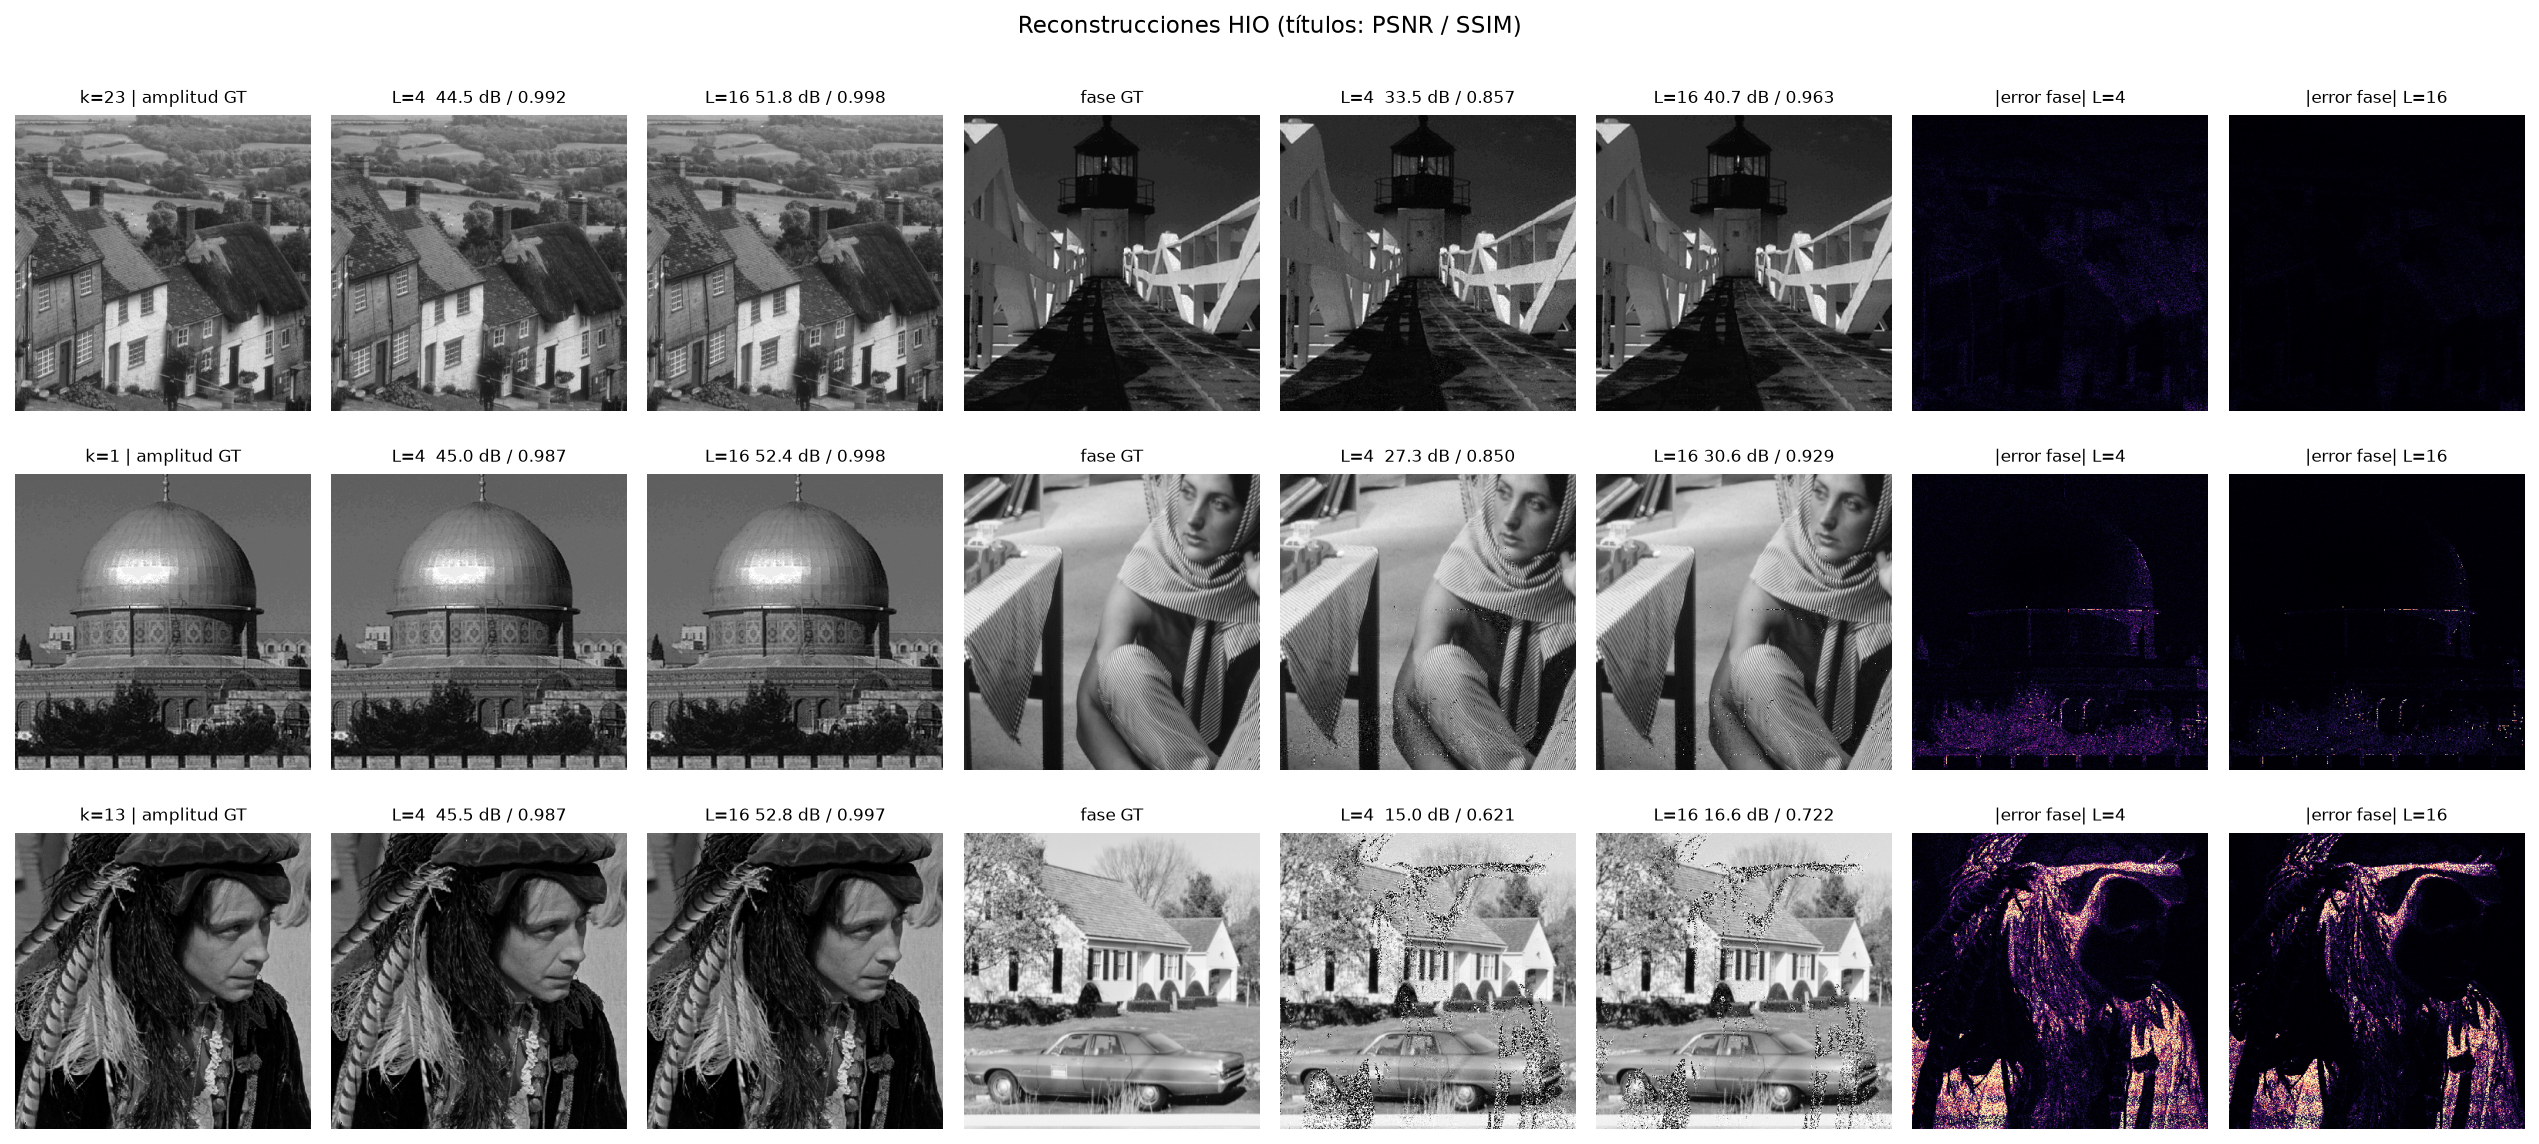
\includegraphics[width=\linewidth]{Fig/visual_examples.png}
    \caption{Reconstrucciones de amplitud y fase con $L=4$ y $L=16$ para los objetos 23, 1 y 13 (títulos: PSNR / SSIM). Las dos últimas columnas muestran el error absoluto de fase.}
    \label{fig:visual}
\end{figure}

\subsection{Error de fase y amplitud del objeto}

La Figura~\ref{fig:error-amp} relaciona el error de fase por píxel con la amplitud real, agregando los 24 objetos. Donde $|\Obj|<0.05$, el RMSE de fase es $\approx0.3$ rad para ambas configuraciones: allí casi no llega luz al sensor y la fase no es observable. En zonas bien iluminadas, el RMSE baja a $\approx0.010$ rad con $L=4$ y $\approx0.0045$ rad con $L=16$, un factor $\approx2.3$.

\begin{figure}[H]
    \centering
    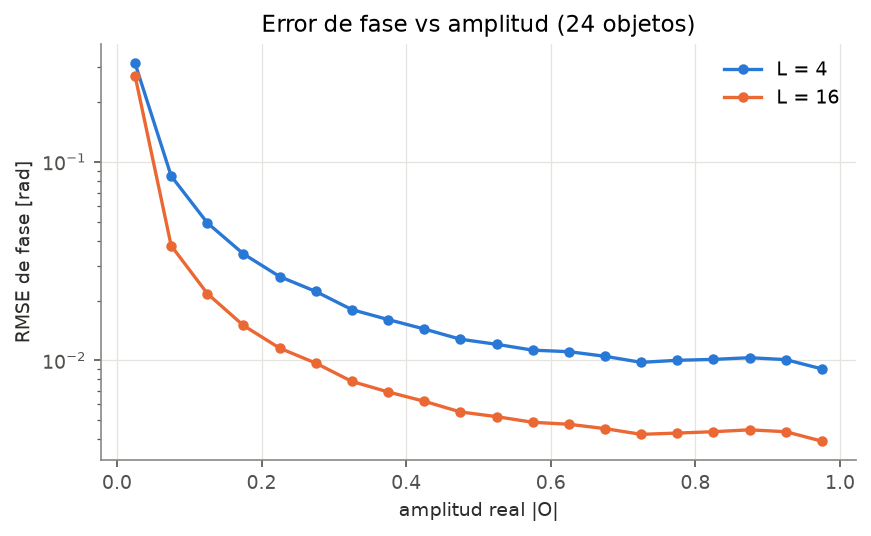
\includegraphics[width=0.72\linewidth]{Fig/phase_error_vs_amplitude.png}
    \caption{RMSE de fase en función de la amplitud real del píxel (24 objetos, SNR $=40$ dB).}
    \label{fig:error-amp}
\end{figure}

Este efecto explica casi toda la dispersión de la PSNR de fase entre imágenes. La correlación de Spearman entre la fracción de píxeles de amplitud menor que $0.05$ y la PSNR de fase es $\rho=-0.92$ con $L=4$ y $\rho=-0.89$ con $L=16$.

\subsection{Imágenes más y menos favorables}

Con $L=4$, la mejor fase corresponde a $k=23$, con $33.55$ dB y SSIM $0.857$; su amplitud (imagen 2) casi no tiene zonas oscuras. Las peores son $k=13$, con $15.01$ dB y SSIM $0.621$, y $k=6$, con $16.25$ dB. Sus amplitudes, las imágenes 12 y 19, tienen un 23\,\% y un 15.5\,\% de píxeles con valor menor que $0.05$. Con $L=16$ el orden se mantiene ($k=23$: $40.67$ dB; $k=13$: $16.57$ dB).

En amplitud ocurre lo contrario: los peores casos son $k=14$ ($40.00$ dB con $L=4$, $47.21$ dB con $L=16$) y $k=15$ ($40.24$ / $47.50$ dB), cuyas amplitudes (imágenes 11 y 10) son las más brillantes del dataset, con media $0.75$ y $0.73$. Como el ruido se define con un SNR relativo, su magnitud absoluta crece con la intensidad, y la PSNR, que usa $\operatorname{MAX}_I=1$ fijo, lo penaliza. La correlación de Spearman entre el brillo medio de la amplitud y la PSNR de amplitud es $\rho=-0.70$. Esos mismos objetos tienen una de las mejores fases ($\rho=+0.82$ entre brillo medio y PSNR de fase): más luz hace la fase más observable.

\subsection{Experimento complementario sin ruido}

Sin ruido, el problema es consistente y el error puede llegar a cero. Esto aísla el efecto de $L$ sobre la velocidad de convergencia (Tabla~\ref{tab:sin-ruido} y Figura~\ref{fig:convergencia-sin-ruido}). Se reportan medianas y rangos porque, en reconstrucciones casi exactas, la PSNR puede superar los 200 dB y distorsionar la media.

\begin{table}[H]
\centering
\caption{Resultados sin ruido con 100 iteraciones: mediana (mínimo -- máximo) sobre las 24 imágenes.}
\label{tab:sin-ruido}
\small
\begin{tabular}{lrr}
\toprule
Métrica & $L=4$ & $L=16$ \\
\midrule
PSNR amplitud (dB) & $87.09$ ($81.77$ -- $89.96$) & $235.54$ ($223.04$ -- $237.89$) \\
PSNR fase (dB) & $31.54$ ($17.33$ -- $76.18$) & $31.83$ ($17.43$ -- $224.52$) \\
SSIM fase & $0.9794$ ($0.8134$ -- $1.0000$) & $0.9810$ ($0.8162$ -- $1.0000$) \\
$E_k$ final (mediana) & $4.19\times10^{-5}$ & $3.24\times10^{-12}$ \\
\midrule
Iteraciones hasta PSNR amp.\ $\geq40$ dB & 15 (24/24) & 8 (24/24) \\
Iteraciones hasta PSNR amp.\ $\geq60$ dB & 34 (24/24) & 15 (24/24) \\
Iteraciones hasta PSNR amp.\ $\geq100$ dB & 86 (10/24) & 34 (24/24) \\
\bottomrule
\end{tabular}
\end{table}

\begin{figure}[H]
    \centering
    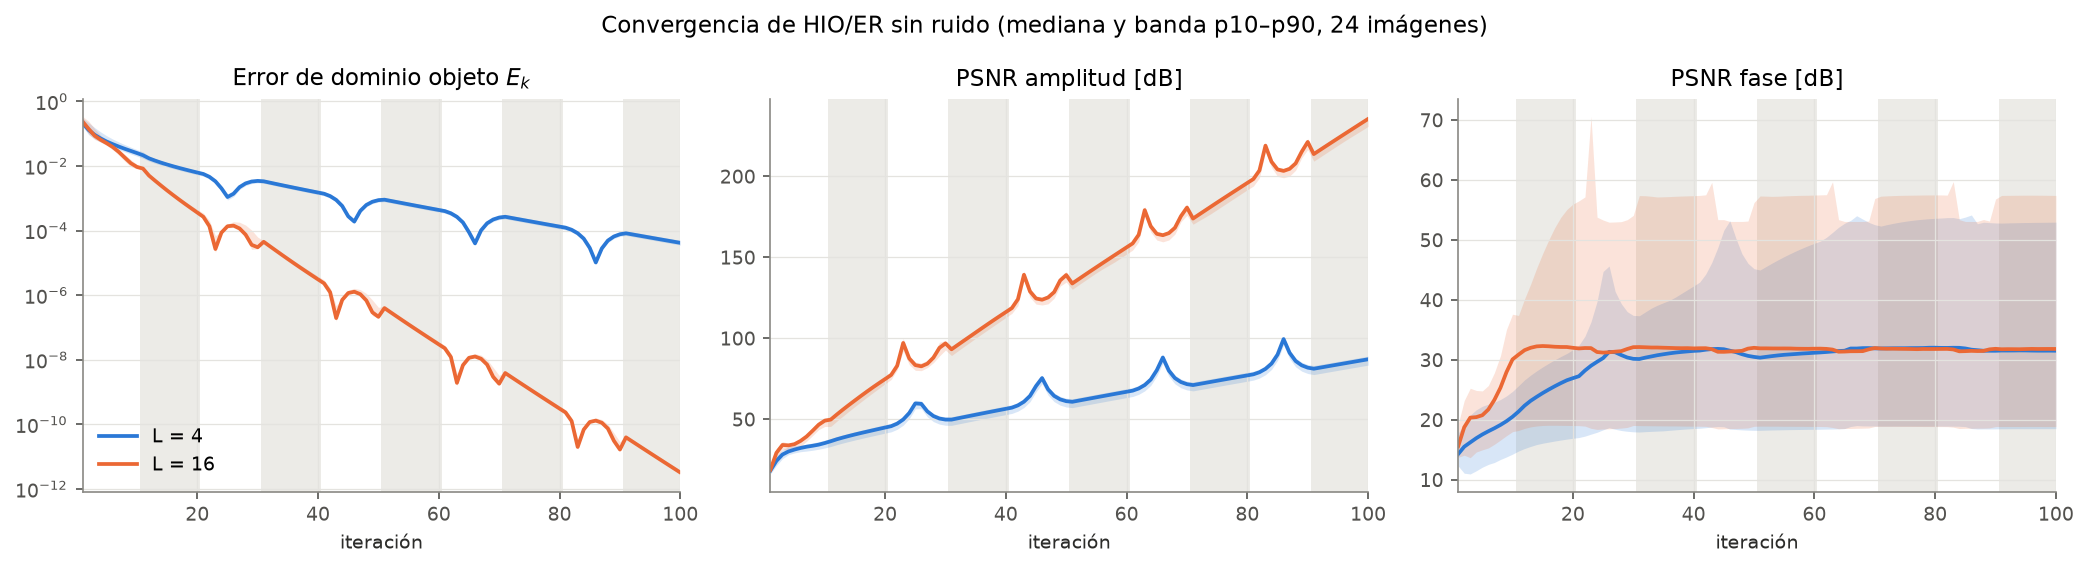
\includegraphics[width=\linewidth]{Fig/convergence_sin_ruido.png}
    \caption{Convergencia de \hio{}/\er{} sin ruido. Con $L=16$, $E_k$ decrece aproximadamente de forma lineal en escala logarítmica hasta la precisión de máquina; con $L=4$ la tasa es mucho menor.}
    \label{fig:convergencia-sin-ruido}
\end{figure}

Con $L=16$, $E_k$ llega a $\sim10^{-12}$ (precisión de máquina) en 100 iteraciones, mientras que con $L=4$ se queda en $\sim10^{-5}$. En cambio, la mediana de la PSNR de fase es casi idéntica (31.5 frente a 31.8 dB): sin ruido, la fase solo se recupera de forma casi exacta en los objetos cuya amplitud no se anula, y eso no depende de $L$.

\subsection{Robustez frente al nivel y al tipo de ruido}
\label{sec:robustez}

Como el protocolo principal usa un solo nivel de ruido, se repitió el experimento completo (24 objetos, 100 iteraciones, $\beta=0.9$, mismas máscaras y semillas) con SNR gaussiano de $20$, $30$, $40$ y $50$ dB y con ruido de Poisson con $10^3$ y $10^4$ fotones en el pico de intensidad, es decir, $Y_\ell\leftarrow\mathrm{Poisson}(Y_\ell\,n_\mathrm{pico}/\max Y)\,\max Y/n_\mathrm{pico}$. Los resultados se obtuvieron con el script \texttt{experimentos\_extra.py}; el caso de $40$ dB reproduce exactamente la Tabla~\ref{tab:resumen}, lo que verifica que el pipeline es el mismo.

\begin{table}[H]
\centering
\caption{Media sobre las 24 imágenes para distintos niveles y tipos de ruido.}
\label{tab:robustez}
\small
\begin{tabular}{llrrrr}
\toprule
Ruido & $L$ & PSNR amp.\ (dB) & SSIM amp. & PSNR fase (dB) & SSIM fase \\
\midrule
Gauss $20$ dB & 4  & $23.76$ & $0.591$ & $12.72$ & $0.245$ \\
              & 16 & $33.75$ & $0.897$ & $19.01$ & $0.564$ \\
Gauss $30$ dB & 4  & $35.00$ & $0.917$ & $19.85$ & $0.603$ \\
              & 16 & $42.47$ & $0.981$ & $24.59$ & $0.794$ \\
Gauss $40$ dB & 4  & $44.10$ & $0.987$ & $25.57$ & $0.823$ \\
              & 16 & $51.39$ & $0.997$ & $29.10$ & $0.904$ \\
Gauss $50$ dB & 4  & $53.20$ & $0.998$ & $29.78$ & $0.915$ \\
              & 16 & $60.51$ & $1.000$ & $31.96$ & $0.940$ \\
\midrule
Poisson $10^3$ fotones & 4  & $32.53$ & $0.873$ & $18.32$ & $0.523$ \\
                       & 16 & $39.90$ & $0.969$ & $23.10$ & $0.739$ \\
Poisson $10^4$ fotones & 4  & $43.01$ & $0.984$ & $25.01$ & $0.805$ \\
                       & 16 & $50.02$ & $0.997$ & $28.56$ & $0.895$ \\
\bottomrule
\end{tabular}
\end{table}

\begin{figure}[H]
    \centering
    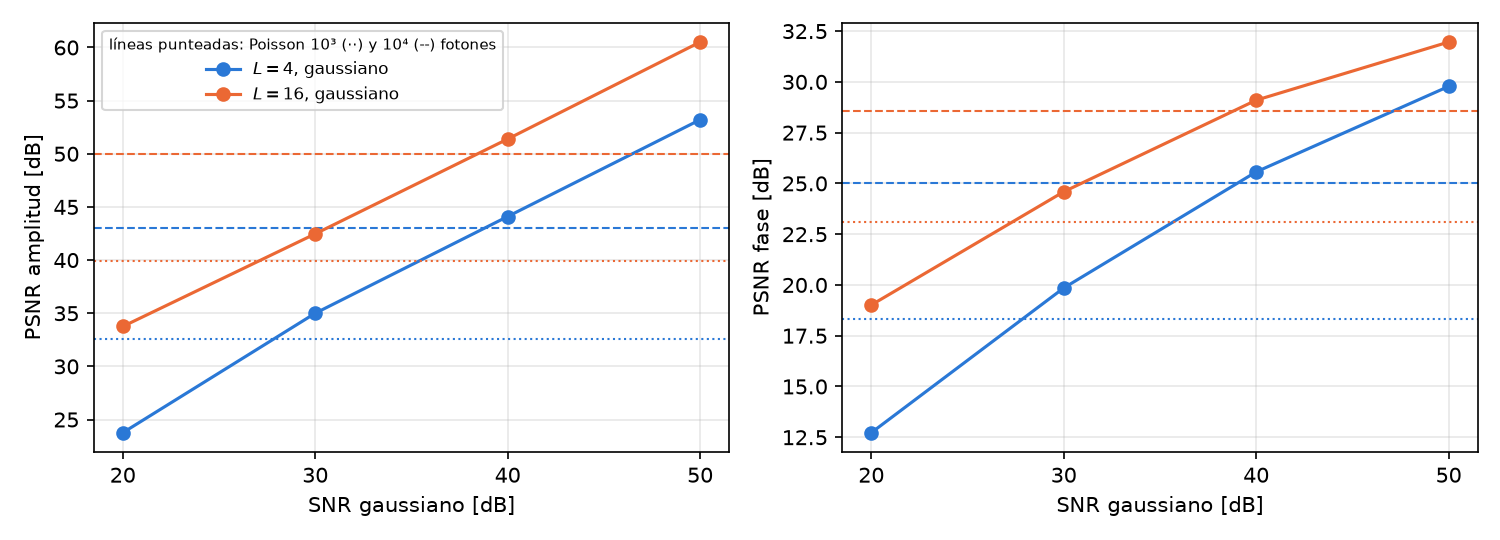
\includegraphics[width=\linewidth]{Fig/extra_ruido.png}
    \caption{PSNR media de amplitud y de fase frente al SNR gaussiano. Las líneas horizontales indican los resultados con ruido de Poisson ($10^3$ y $10^4$ fotones).}
    \label{fig:robustez}
\end{figure}

Se observan cuatro hechos. Primero, la PSNR de amplitud crece aproximadamente $0.9$--$1.1$ dB por cada dB de SNR: el error de reconstrucción es proporcional al nivel de ruido, lo esperable en un problema bien condicionado. Segundo, $L=16$ supera a $L=4$ en todos los niveles y tipos de ruido. La ventaja en amplitud es de $10.0$, $7.5$, $7.3$ y $7.3$ dB para $20$, $30$, $40$ y $50$ dB, y la de fase pasa de $6.3$ dB a $2.2$ dB al bajar el ruido. Tercero, con SNR bajo la fase se degrada mucho más que la amplitud: con $20$ dB y $L=4$ el SSIM de fase cae a $0.245$. Cuarto, el ruido de Poisson, cuya varianza depende de la intensidad, da resultados comparables al gaussiano de SNR equivalente: $10^4$ fotones queda cerca del caso de $40$ dB ($43.0$ frente a $44.1$ dB con $L=4$) y $10^3$ fotones equivale, por interpolación lineal en la Tabla~\ref{tab:robustez}, a unos $28$ dB gaussianos. Por lo tanto, la conclusión principal no depende del modelo de ruido elegido.

\section{Discusión}

\subsection{Por qué \texorpdfstring{$L=16$}{L=16} mejora la reconstrucción}

La mejora no proviene de cambiar el objeto, el ruido por medición ni el algoritmo: ambas configuraciones usan el mismo dataset, el mismo SNR, el mismo $\beta$ y el mismo número de iteraciones. Lo que cambia es la cantidad de información medida. Con máscaras complementarias, cada píxel del objeto aparece en $L/2$ mediciones: 2 con $L=4$ y 8 con $L=16$. Con el mismo SNR por medición, cuadruplicar la redundancia promedia el ruido. Para un estimador de mínimos cuadrados cabría esperar una ganancia de $10\log_{10}4\approx6$ dB; la ganancia observada en amplitud ($+7.3$ dB) es algo mayor, lo que sugiere que las mediciones adicionales también mejoran el condicionamiento del problema no lineal. La reducción del RMSE de fase en zonas iluminadas en un factor $\approx2.3\approx\sqrt{4}$ es consistente con el mismo argumento.

La velocidad de convergencia responde a la misma causa. Más máscaras implican más restricciones independientes sobre el mismo objeto, el conjunto de soluciones compatibles con las mediciones se reduce y cada iteración avanza más. El efecto es particularmente claro sin ruido, donde $L=16$ reduce $E_k$ siete órdenes de magnitud más que $L=4$ en las mismas 100 iteraciones.

\subsection{Por qué \hio{} puro falla con ruido}

\hio{} está pensado para problemas consistentes: su punto fijo es una solución que satisface ambas restricciones. Con ruido, esa solución no existe, y el término de realimentación $(I-P_\mathcal{S})(g_k-\beta g'_k)$ acumula sin límite la componente que no puede anularse. La estimación $P_\mathcal{S}(g'_k)$ se degrada progresivamente (Figura~\ref{fig:ablation}). Alternar bloques \er{} reinicia esa componente periódicamente y conserva la ventaja de \hio{}: en este problema, llegar al nivel final casi al doble de velocidad que \er{}. Una alternativa diseñada para el caso inconsistente sería RAAR \cite{luke2005raar}, que queda fuera del alcance de la tarea.

\subsection{Un error \texorpdfstring{$E_k$}{Ek} mayor no significa peor reconstrucción}

El piso de $E_k$ con ruido es algo mayor con $L=16$ ($1.47\times10^{-2}$) que con $L=4$ ($1.11\times10^{-2}$), aunque la reconstrucción con $L=16$ es claramente mejor. $E_k$ mide la inconsistencia entre las mediciones ruidosas y el conjunto de restricciones, no el error respecto del objeto real. Con 16 mediciones ruidosas hay más inconsistencias que no pueden satisfacerse a la vez. Por eso $E_k$ sirve como criterio de convergencia, pero no para comparar configuraciones con distinto $L$.

\subsection{Costo computacional y de adquisición}

El costo por iteración crece de forma aproximadamente lineal con $L$: $14.8$ ms frente a $52.7$ ms ($\approx3.6\times$), porque cada iteración propaga y retropropaga las $L$ ondas. Los tiempos absolutos dependen del equipo; la razón entre configuraciones es estable. Medido hasta la convergencia, $L=4$ es más barato ($25\times14.8$ ms $\approx0.37$ s) que $L=16$ ($15\times52.7$ ms $\approx0.79$ s), pero converge a una calidad bastante menor. En un sistema real, $L=16$ también requiere 4 veces más capturas con el DMD. La elección entre ambos es, por tanto, una disyuntiva entre calidad y tiempo de adquisición y cómputo.

\subsection{Limitaciones del análisis}

\begin{itemize}
    \item La fase toma valores en $[0,1]$ rad, como en \texttt{main.m}. Es un objeto de fase débil, sin \emph{wrapping}; fases en $[0,2\pi)$ requerirían, además, desenvolver la fase.
    \item El experimento principal usa ruido gaussiano aditivo con SNR de $40$ dB. La Sección~\ref{sec:robustez} lo complementa con otros SNR y con ruido de Poisson, pero no se modelan otros efectos del sensor (cuantización, saturación, ruido de lectura).
    \item La alineación de fase global usa el objeto real. Es la práctica habitual para evaluar, pero no está disponible en un experimento real.
    \item Solo se evaluaron máscaras aleatorias y una distancia de propagación. El enunciado menciona que otras familias de máscaras, como las de Hadamard, reducen la correlación entre mediciones; no se estudiaron aquí.
    \item Las amplitudes normalizadas con \texttt{mat2gray} contienen píxeles exactamente nulos. Allí la fase no está definida, lo que acota la PSNR de fase independientemente del algoritmo.
\end{itemize}

\section{Conclusiones}

Se portó a Python el laboratorio de recuperación de fase: modelo directo, máscaras complementarias y propagador de espectro angular. El port coincide con el original a precisión de máquina y es unas 11 veces más rápido gracias a una reformulación exacta del propagador multipaso. El esquema de reconstrucción del repositorio se reemplazó por el algoritmo Hybrid Input--Output, extendido a $L$ aperturas codificadas mediante una proyección de consenso que las máscaras complementarias hacen siempre bien definida.

Con datos ruidosos, \hio{} puro diverge. Alternar bloques de \hio{} y \er{} lo estabiliza y, además, alcanza el nivel final casi el doble de rápido que \er{}, que es el esquema implícito en \texttt{PhaseLiftSimu.m}.

Con $L=4$ ya se recupera la amplitud con alta fidelidad: $44.10$ dB y SSIM $0.987$ en promedio. Pasar a $L=16$ mejora la amplitud en $7.29$ dB y la fase en $3.53$ dB, eleva el SSIM de fase de $0.823$ a $0.904$ y reduce las iteraciones necesarias de 25 a 15. Sin ruido, la diferencia de velocidad es aún mayor. La mejora se observa en las 24 imágenes y en las cuatro métricas, y se explica por la mayor redundancia: cada píxel se observa 8 veces en lugar de 2. El costo es 4 veces más mediciones y $\approx3.6$ veces más cómputo por iteración.

La ventaja de $L=16$ se mantiene entre $20$ y $50$ dB de SNR y con ruido de Poisson, y es mayor cuando hay más ruido. La principal limitación restante es la fase en regiones de amplitud casi nula. Su error no depende de $L$ y explica la mayor parte de la dispersión entre imágenes ($\rho=-0.92$). Por lo tanto, para este protocolo, $L=16$ es claramente preferible cuando la calidad de la fase es prioritaria, y $L=4$ es una alternativa razonable cuando el tiempo de adquisición domina y basta con recuperar bien la amplitud.

\section{Material complementario}

El material computacional que acompaña este informe se encuentra en el notebook
\begin{center}
\texttt{tareas/tarea-06/homework6.ipynb}.
\end{center}
El notebook contiene el port del propagador (versión literal y versión precalculada) con sus verificaciones, la generación de máscaras complementarias, la simulación de mediciones, la función \texttt{hio\_reconstruct}, la implementación de PSNR y SSIM según las Ecs.~(5)--(7) del enunciado, el estudio del esquema y de $\beta$, los experimentos con $L=4$ y $L=16$ con y sin ruido, y todas las figuras de este informe. Las métricas por imagen se exportan a \url{tareas/tarea-06/results/metrics_L4.csv} y \url{tareas/tarea-06/results/metrics_L16.csv}, y sus versiones sin ruido a los archivos \texttt{*\_sin\_ruido.csv}. Los experimentos de robustez al ruido (Sección~\ref{sec:robustez}) se generan con \texttt{tareas/tarea-06/experimentos\_extra.py}, que usa \texttt{experimentos\_extra\_lib.py} (funciones copiadas del notebook) y escribe \texttt{results/extra\_*.csv} y \texttt{results/extra\_summary.md}.

Durante el desarrollo se utilizó Claude Code de Anthropic como herramienta de apoyo para portar el código MATLAB, implementar y depurar la reconstrucción, organizar la explicación matemática y preparar las visualizaciones \cite{claude-code}. Esta herramienta no sustituye la revisión del autor: las fórmulas, el código, los valores tabulados y las conclusiones fueron contrastados con la ejecución del notebook y con las referencias citadas en este informe.

% -----------------------------------------------------------------------------
% Bibliografía: se cierra el cuerpo principal antes de comenzar los anexos.
% -----------------------------------------------------------------------------
\clearpage
\renewcommand{\refname}{Referencias}
\bibliographystyle{apalike}
\bibliography{Referencias}
\newpage

\appendix
\section{Anexos}
\label{app:anexos}

\subsection{Tabla final de resultados por imagen}
\label{app:tabla-final}

Este anexo contiene la salida final de los experimentos con ruido (SNR $=40$ dB, 100 iteraciones \hio{}/\er{}). Cada fila corresponde a un objeto $k$, con la fase dada por la imagen $k$ y la amplitud por la imagen $25-k$. Los valores se redondean a cuatro decimales a partir de los archivos exportados por el notebook.

\begin{landscape}
\centering
\scriptsize
\setlength{\tabcolsep}{4pt}
\renewcommand{\arraystretch}{1.05}
\captionof{table}{Resultados por objeto para $L=4$ y $L=16$ (SNR $=40$ dB).}
\label{tab:por-imagen}
\resizebox{0.95\linewidth}{!}{%
\begin{tabular}{r r r r r r r r r r r r r}
\toprule
$k$ & Fase & Amp. & \multicolumn{4}{c}{$L=4$} & \multicolumn{4}{c}{$L=16$} & \multicolumn{2}{c}{Tiempo (s)}\\
\cmidrule(lr){4-7}\cmidrule(lr){8-11}\cmidrule(lr){12-13}
 & img & img & PSNR amp. & SSIM amp. & PSNR fase & SSIM fase & PSNR amp. & SSIM amp. & PSNR fase & SSIM fase & $L=4$ & $L=16$\\
\midrule
%%TABLA_RUIDO%%
1 & 1 & 24 & 45.0040 & 0.9867 & 27.3163 & 0.8497 & 52.3691 & 0.9975 & 30.5510 & 0.9287 & 1.54 & 6.19 \\
2 & 2 & 23 & 45.3852 & 0.9843 & 23.4868 & 0.7674 & 52.6759 & 0.9970 & 30.0353 & 0.9032 & 1.76 & 5.25 \\
3 & 3 & 22 & 44.7375 & 0.9874 & 31.5316 & 0.8822 & 52.0589 & 0.9976 & 33.1688 & 0.9619 & 1.49 & 5.18 \\
4 & 4 & 21 & 46.5893 & 0.9921 & 27.1774 & 0.8634 & 53.8815 & 0.9985 & 28.8149 & 0.9339 & 1.39 & 5.17 \\
5 & 5 & 20 & 42.4400 & 0.9873 & 28.3525 & 0.8713 & 49.7362 & 0.9976 & 33.0154 & 0.9494 & 1.37 & 5.17 \\
6 & 6 & 19 & 45.3732 & 0.9855 & 16.2476 & 0.6630 & 52.6385 & 0.9967 & 17.0708 & 0.7558 & 1.40 & 5.29 \\
7 & 7 & 18 & 42.8913 & 0.9926 & 19.2825 & 0.6480 & 50.1732 & 0.9986 & 21.3450 & 0.7704 & 1.43 & 5.24 \\
8 & 8 & 17 & 44.7790 & 0.9834 & 16.3543 & 0.6822 & 52.1086 & 0.9962 & 17.1478 & 0.7842 & 1.45 & 5.55 \\
9 & 9 & 16 & 43.9314 & 0.9959 & 20.0233 & 0.7172 & 51.2470 & 0.9992 & 20.7757 & 0.7935 & 1.44 & 5.37 \\
10 & 10 & 15 & 46.2006 & 0.9939 & 29.1096 & 0.8603 & 53.4679 & 0.9988 & 31.7472 & 0.9498 & 1.38 & 5.19 \\
11 & 11 & 14 & 45.7810 & 0.9977 & 27.9107 & 0.8880 & 53.1139 & 0.9996 & 29.7942 & 0.9497 & 1.37 & 5.25 \\
12 & 12 & 13 & 41.3485 & 0.9800 & 31.3436 & 0.9198 & 48.6596 & 0.9961 & 38.3413 & 0.9758 & 1.34 & 5.22 \\
13 & 13 & 12 & 45.5198 & 0.9868 & 15.0098 & 0.6212 & 52.8284 & 0.9974 & 16.5663 & 0.7217 & 1.39 & 5.21 \\
14 & 14 & 11 & 39.9989 & 0.9766 & 31.2998 & 0.9487 & 47.2060 & 0.9954 & 37.6778 & 0.9866 & 1.44 & 5.20 \\
15 & 15 & 10 & 40.2370 & 0.9610 & 31.0544 & 0.9339 & 47.5004 & 0.9923 & 37.4627 & 0.9775 & 1.47 & 5.20 \\
16 & 16 & 9 & 43.9725 & 0.9879 & 22.4471 & 0.8501 & 51.3386 & 0.9977 & 24.2531 & 0.9258 & 1.48 & 5.19 \\
17 & 17 & 8 & 43.8689 & 0.9851 & 21.3036 & 0.7164 & 51.1974 & 0.9971 & 25.9158 & 0.8301 & 1.57 & 5.19 \\
18 & 18 & 7 & 40.6468 & 0.9844 & 32.2551 & 0.9522 & 47.8965 & 0.9970 & 37.4152 & 0.9870 & 1.53 & 5.23 \\
19 & 19 & 6 & 46.3512 & 0.9912 & 18.9072 & 0.7986 & 53.5864 & 0.9982 & 19.7399 & 0.8549 & 1.56 & 5.17 \\
20 & 20 & 5 & 44.5421 & 0.9915 & 25.6410 & 0.8834 & 51.7892 & 0.9984 & 28.3490 & 0.9514 & 1.68 & 5.19 \\
21 & 21 & 4 & 44.9288 & 0.9912 & 33.4685 & 0.9176 & 52.1632 & 0.9983 & 37.9020 & 0.9748 & 1.44 & 5.15 \\
22 & 22 & 3 & 46.6493 & 0.9892 & 21.5587 & 0.8267 & 53.9682 & 0.9980 & 24.5586 & 0.9172 & 1.52 & 5.20 \\
23 & 23 & 2 & 44.5351 & 0.9920 & 33.5481 & 0.8565 & 51.7874 & 0.9985 & 40.6701 & 0.9627 & 1.51 & 5.18 \\
24 & 24 & 1 & 42.6709 & 0.9832 & 29.0112 & 0.8360 & 49.9478 & 0.9968 & 36.0614 & 0.9454 & 1.47 & 5.19 \\
\midrule
\multicolumn{3}{l}{Promedio} & 44.0993 & 0.9870 & 25.5684 & 0.8231 & 51.3892 & 0.9974 & 29.0991 & 0.9038 & 1.48 & 5.27 \\
\bottomrule
\end{tabular}%
}
\end{landscape}

\subsection{Resultados por imagen sin ruido}
\label{app:tabla-sin-ruido}

\begin{table}[H]
\centering
\scriptsize
\setlength{\tabcolsep}{4pt}
\caption{Resultados por objeto sin ruido (100 iteraciones \hio{}/\er{}).}
\label{tab:por-imagen-sin-ruido}
\begin{tabular}{r r r r r r r r r}
\toprule
$k$ & \multicolumn{4}{c}{$L=4$} & \multicolumn{4}{c}{$L=16$}\\
\cmidrule(lr){2-5}\cmidrule(lr){6-9}
 & PSNR amp. & SSIM amp. & PSNR fase & SSIM fase & PSNR amp. & SSIM amp. & PSNR fase & SSIM fase\\
\midrule
%%TABLA_SIN_RUIDO%%
1 & 85.97 & 1.0000 & 31.40 & 0.9705 & 236.54 & 1.0000 & 31.90 & 0.9720 \\
2 & 89.96 & 1.0000 & 40.60 & 0.9955 & 237.11 & 1.0000 & 40.55 & 0.9956 \\
3 & 88.13 & 1.0000 & 33.90 & 0.9860 & 235.90 & 1.0000 & 34.53 & 0.9877 \\
4 & 89.68 & 1.0000 & 29.06 & 0.9550 & 237.89 & 1.0000 & 29.76 & 0.9586 \\
5 & 85.70 & 1.0000 & 35.96 & 0.9857 & 234.37 & 1.0000 & 35.51 & 0.9846 \\
6 & 87.66 & 1.0000 & 17.33 & 0.8164 & 235.61 & 1.0000 & 17.43 & 0.8184 \\
7 & 86.34 & 1.0000 & 23.03 & 0.8787 & 234.16 & 1.0000 & 23.49 & 0.8863 \\
8 & 86.59 & 1.0000 & 17.59 & 0.8623 & 234.86 & 1.0000 & 17.59 & 0.8639 \\
9 & 88.38 & 1.0000 & 21.11 & 0.8281 & 236.15 & 1.0000 & 21.23 & 0.8319 \\
10 & 87.82 & 1.0000 & 31.78 & 0.9787 & 236.40 & 1.0000 & 33.51 & 0.9825 \\
11 & 86.37 & 1.0000 & 29.12 & 0.9659 & 235.70 & 1.0000 & 31.20 & 0.9758 \\
12 & 83.26 & 1.0000 & 72.68 & 1.0000 & 232.16 & 1.0000 & 221.62 & 1.0000 \\
13 & 88.54 & 1.0000 & 17.89 & 0.8134 & 235.89 & 1.0000 & 18.25 & 0.8162 \\
14 & 82.98 & 1.0000 & 46.40 & 0.9992 & 230.88 & 1.0000 & 45.55 & 0.9991 \\
15 & 84.01 & 1.0000 & 50.39 & 0.9992 & 232.32 & 1.0000 & 56.02 & 0.9996 \\
16 & 87.00 & 1.0000 & 24.96 & 0.9547 & 230.55 & 1.0000 & 25.07 & 0.9557 \\
17 & 87.51 & 1.0000 & 28.43 & 0.9580 & 223.04 & 1.0000 & 29.03 & 0.9614 \\
18 & 81.77 & 1.0000 & 40.01 & 0.9977 & 230.94 & 1.0000 & 40.01 & 0.9976 \\
19 & 88.41 & 1.0000 & 20.07 & 0.8851 & 236.98 & 1.0000 & 20.39 & 0.8882 \\
20 & 85.48 & 1.0000 & 29.18 & 0.9808 & 235.34 & 1.0000 & 29.27 & 0.9812 \\
21 & 88.34 & 1.0000 & 39.94 & 0.9949 & 236.02 & 1.0000 & 41.03 & 0.9958 \\
22 & 89.24 & 1.0000 & 31.68 & 0.9802 & 237.42 & 1.0000 & 31.77 & 0.9807 \\
23 & 87.18 & 1.0000 & 76.18 & 1.0000 & 235.47 & 1.0000 & 224.52 & 1.0000 \\
24 & 85.55 & 1.0000 & 54.09 & 0.9997 & 234.41 & 1.0000 & 58.05 & 0.9999 \\
\bottomrule
\end{tabular}
\end{table}

\subsection{Comparaciones visuales de las 24 reconstrucciones}
\label{app:visual}

Las siguientes láminas reúnen la comparación completa del dataset con ruido de $40$ dB. Cada fila corresponde a un objeto $k$ y muestra, de izquierda a derecha, la amplitud real, la amplitud reconstruida con $L=4$ y con $L=16$, la fase real y la fase reconstruida con $L=4$ y con $L=16$; los títulos indican PSNR / SSIM. Las láminas se generan en la última sección del notebook.

\begin{landscape}
\begin{figure}[H]
    \centering
    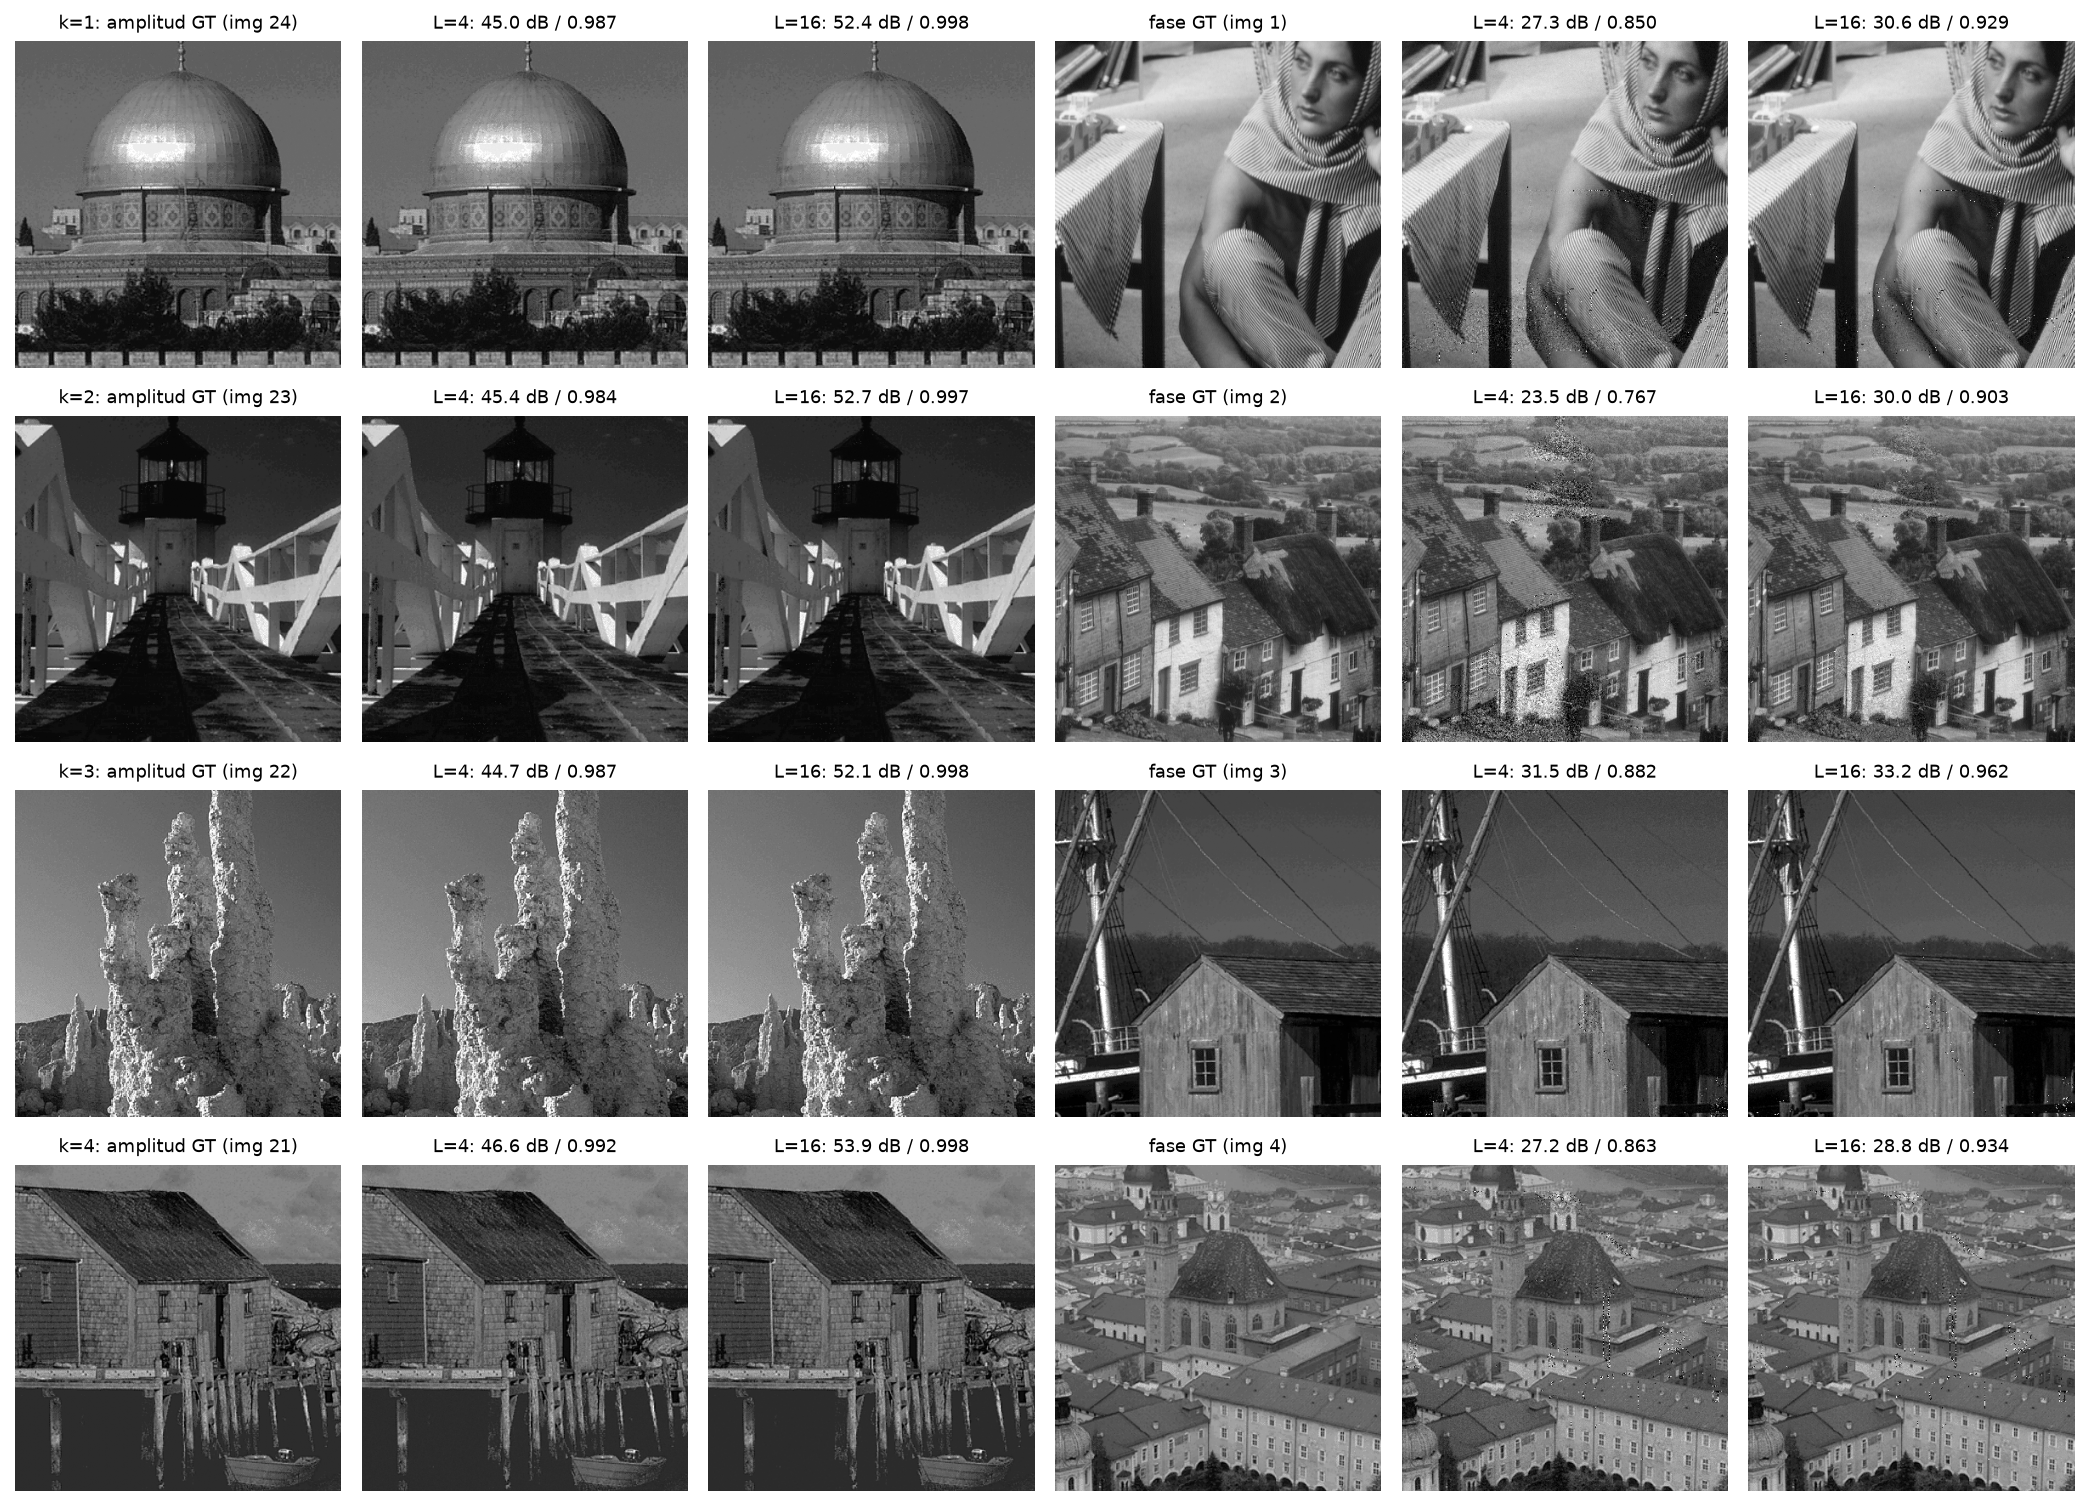
\includegraphics[height=0.78\textheight,keepaspectratio]{Fig/anexo_comparaciones_01_04.png}
    \caption{Reconstrucciones de los objetos 1--4.}
    \label{fig:anexo-01-04}
\end{figure}

\clearpage
\begin{figure}[H]
    \centering
    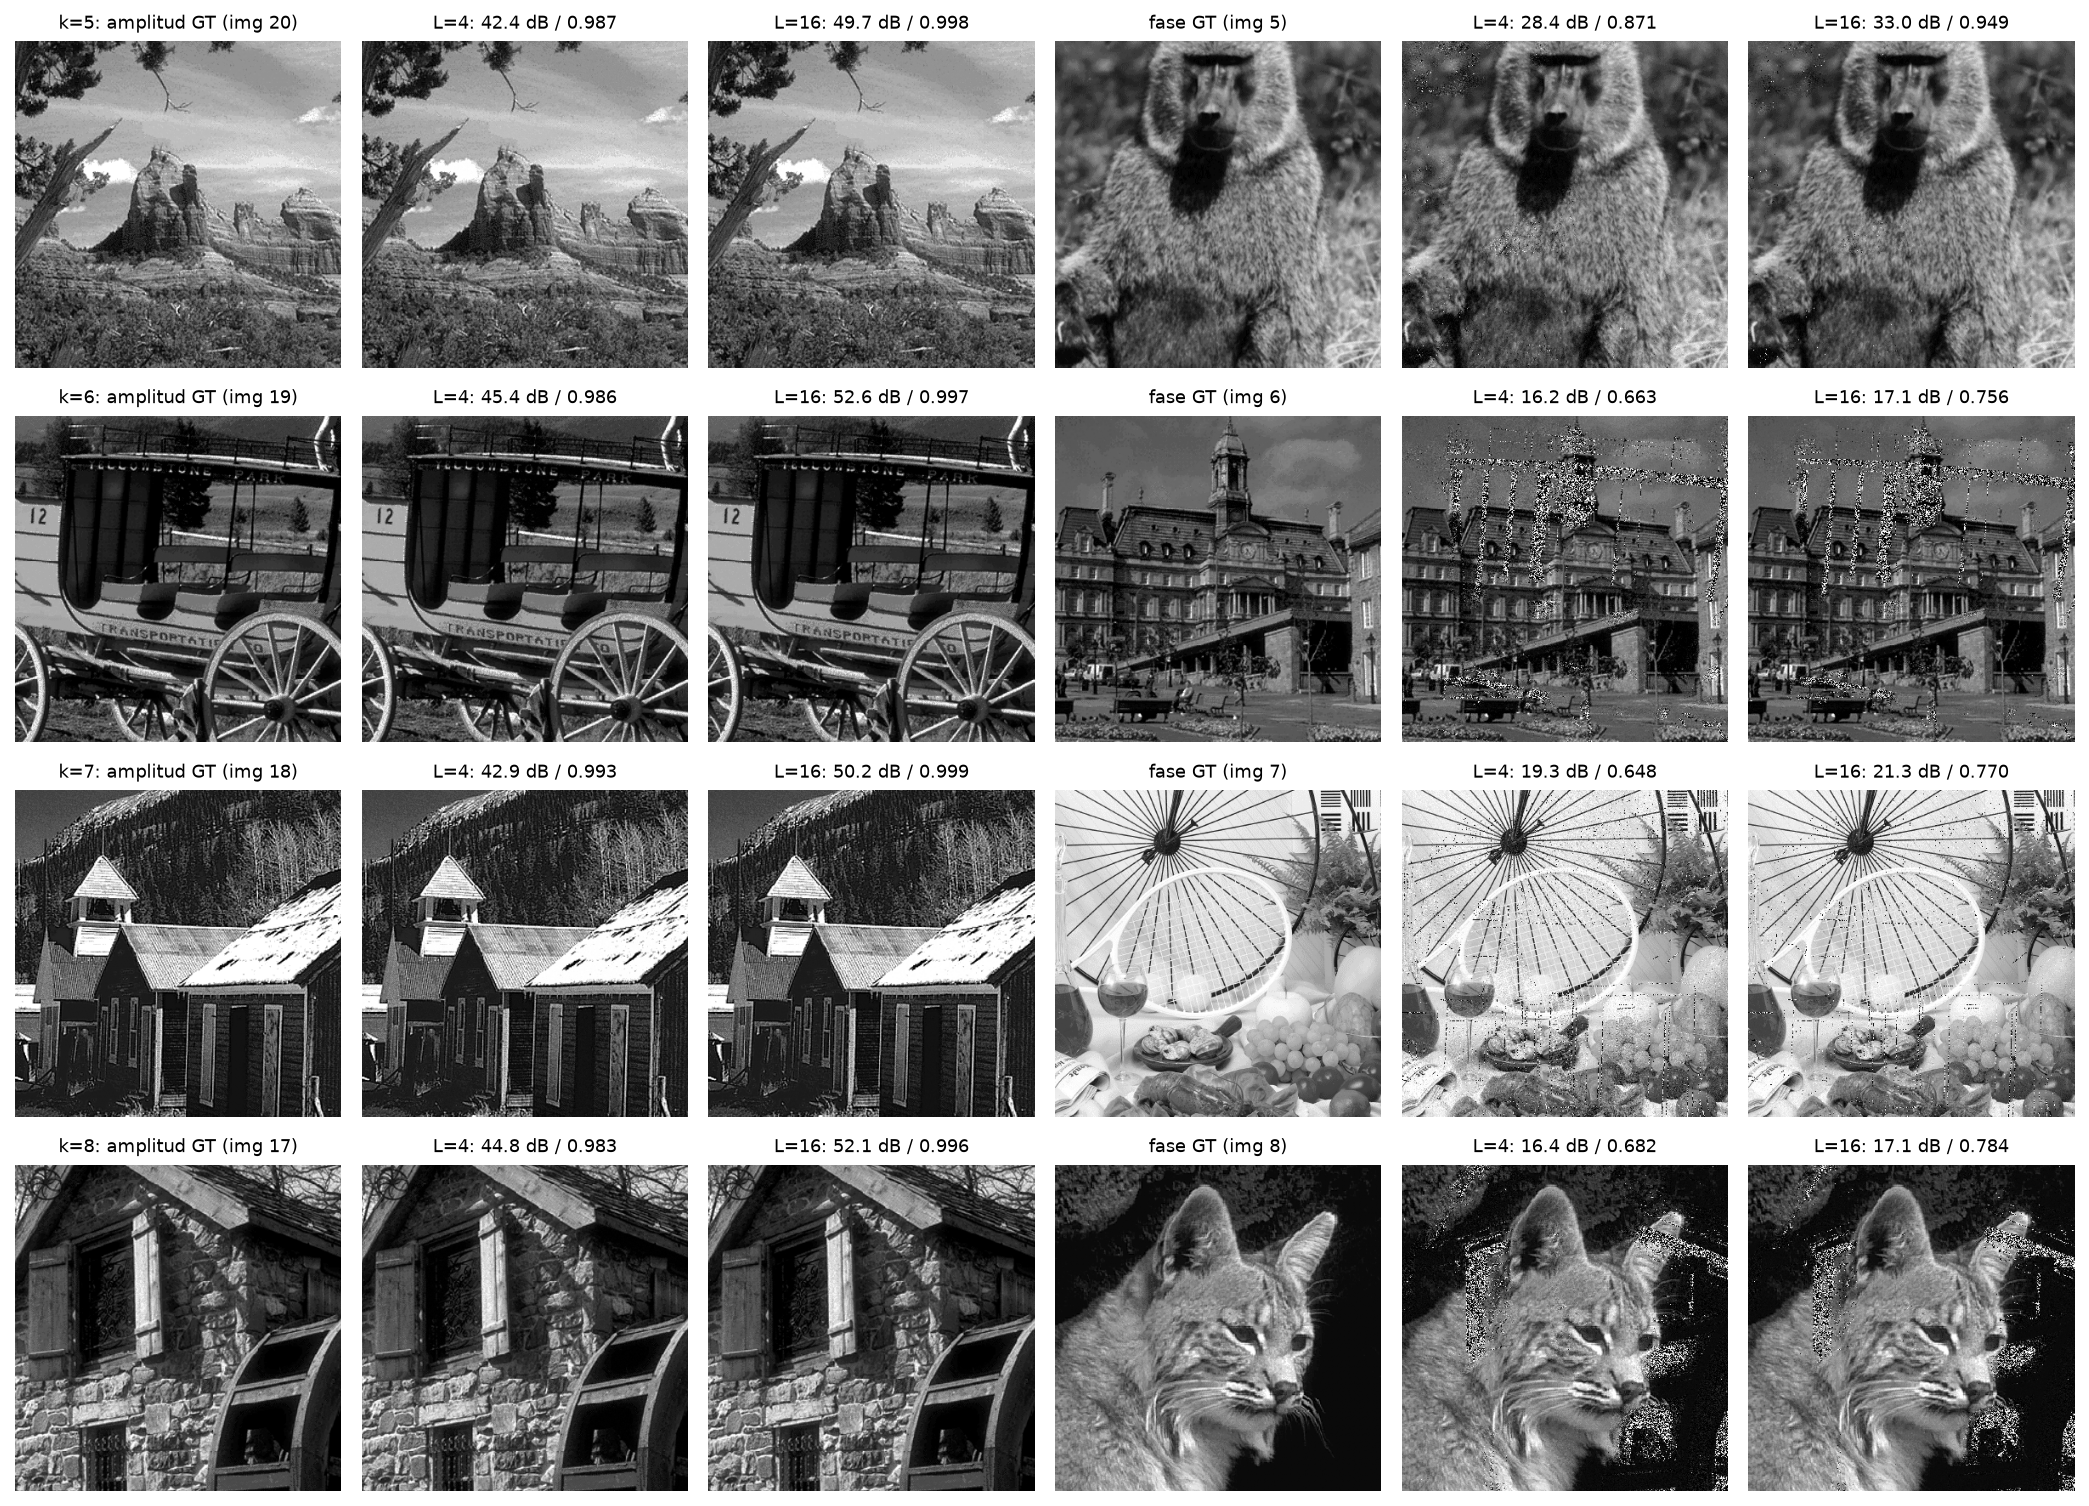
\includegraphics[height=0.78\textheight,keepaspectratio]{Fig/anexo_comparaciones_05_08.png}
    \caption{Reconstrucciones de los objetos 5--8.}
    \label{fig:anexo-05-08}
\end{figure}

\clearpage
\begin{figure}[H]
    \centering
    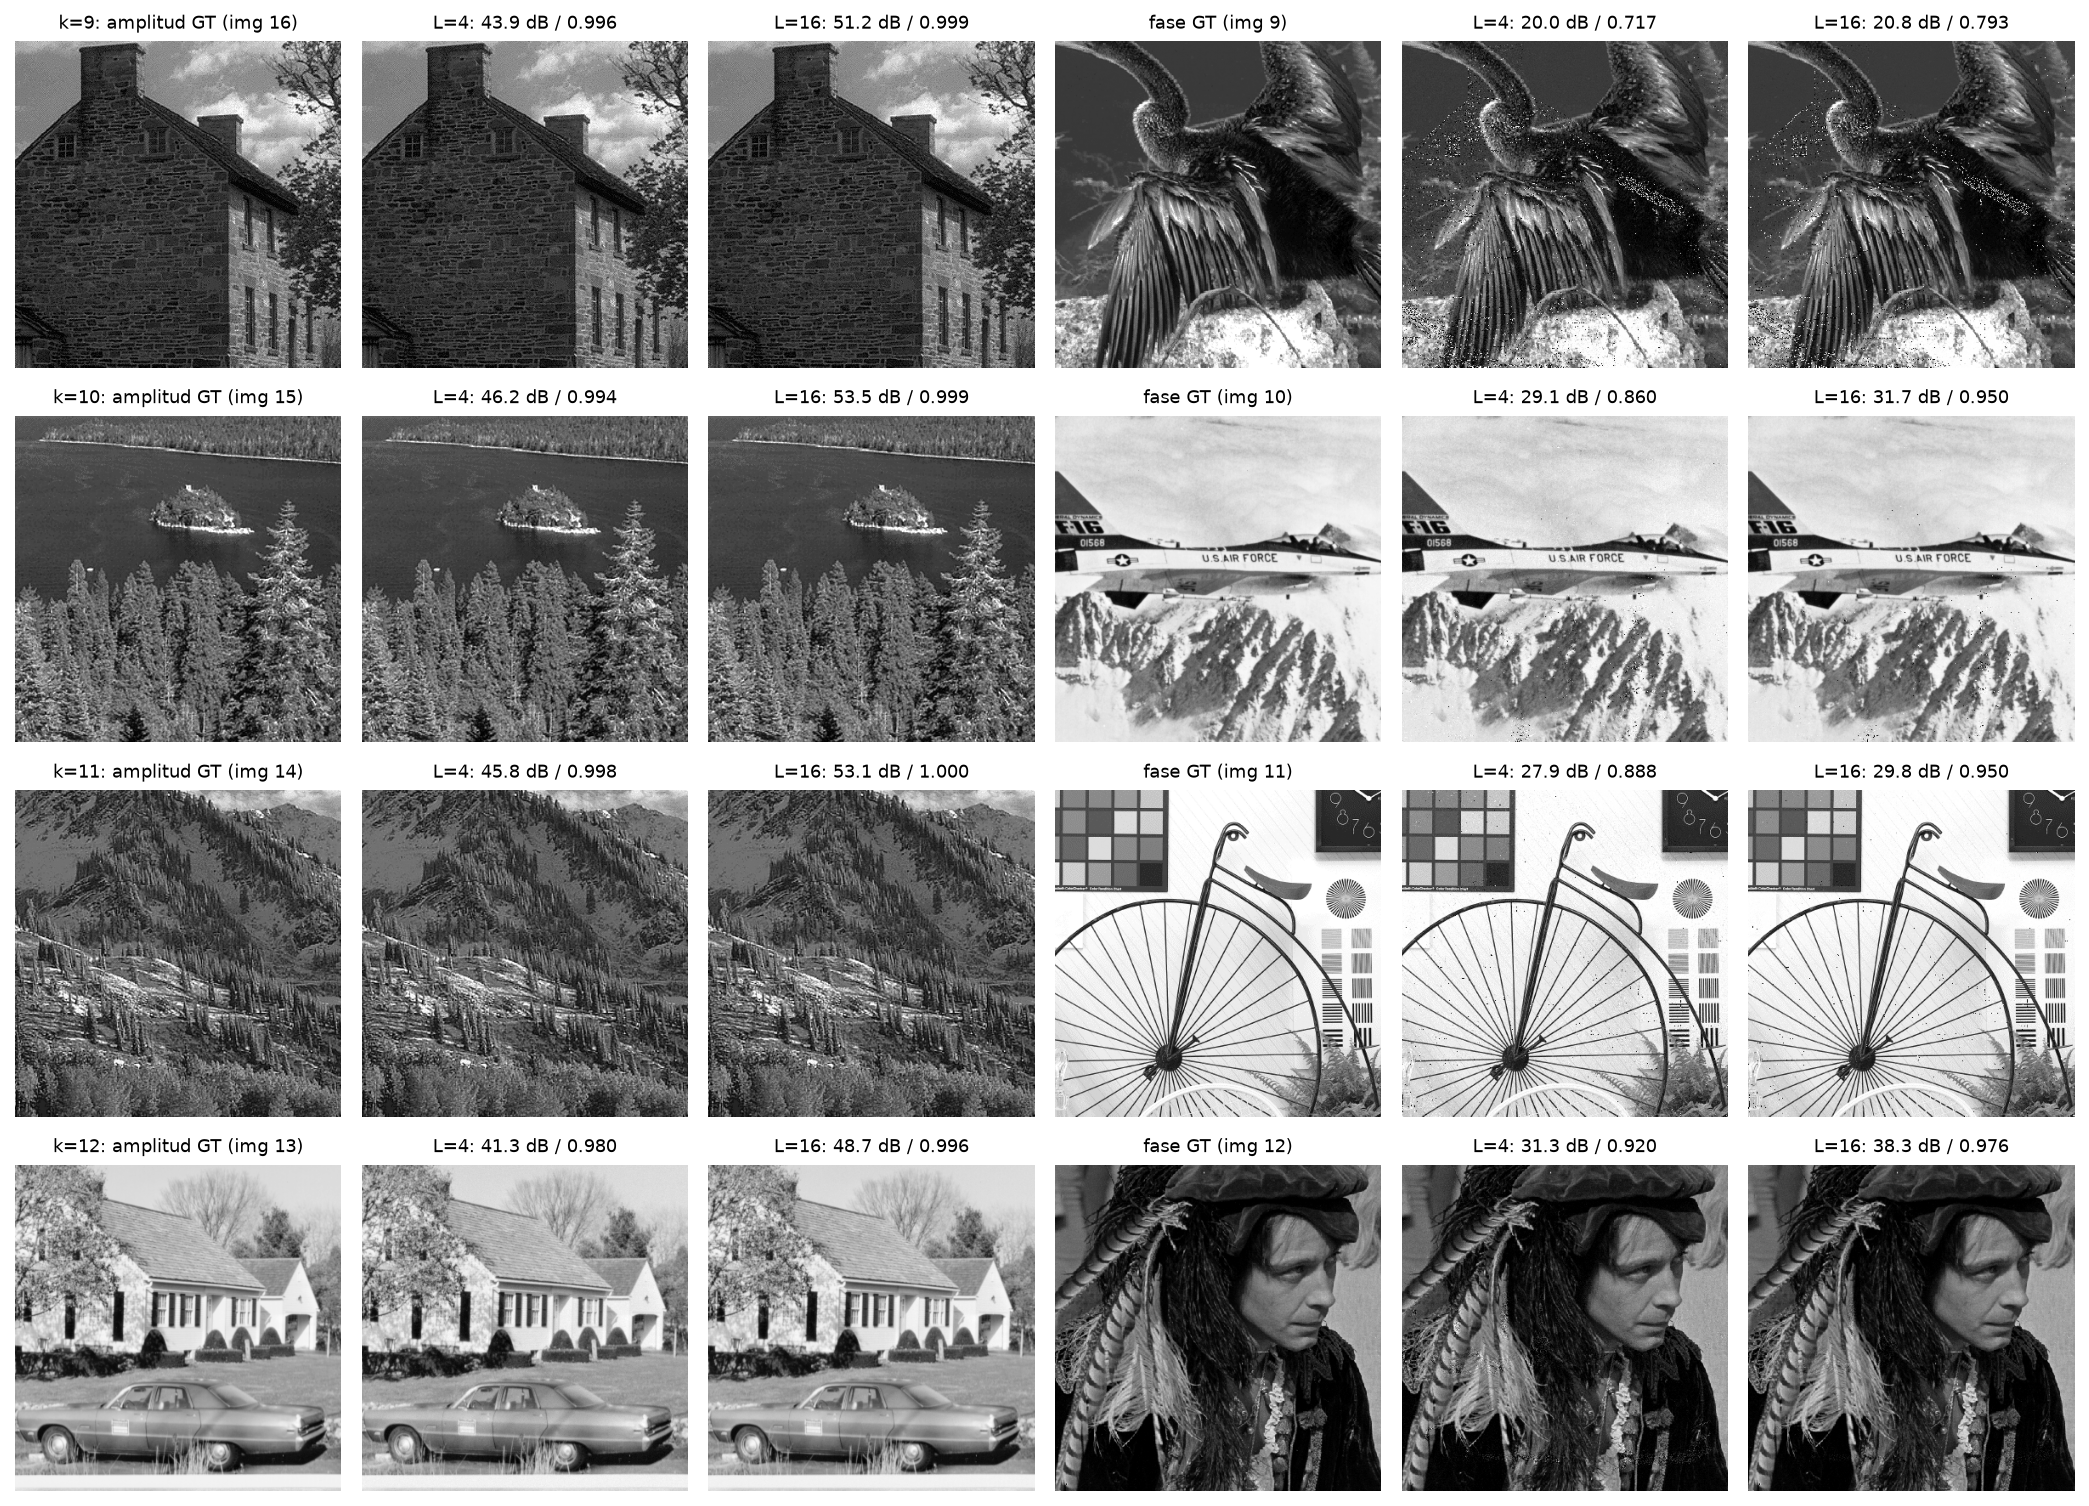
\includegraphics[height=0.78\textheight,keepaspectratio]{Fig/anexo_comparaciones_09_12.png}
    \caption{Reconstrucciones de los objetos 9--12.}
    \label{fig:anexo-09-12}
\end{figure}

\clearpage
\begin{figure}[H]
    \centering
    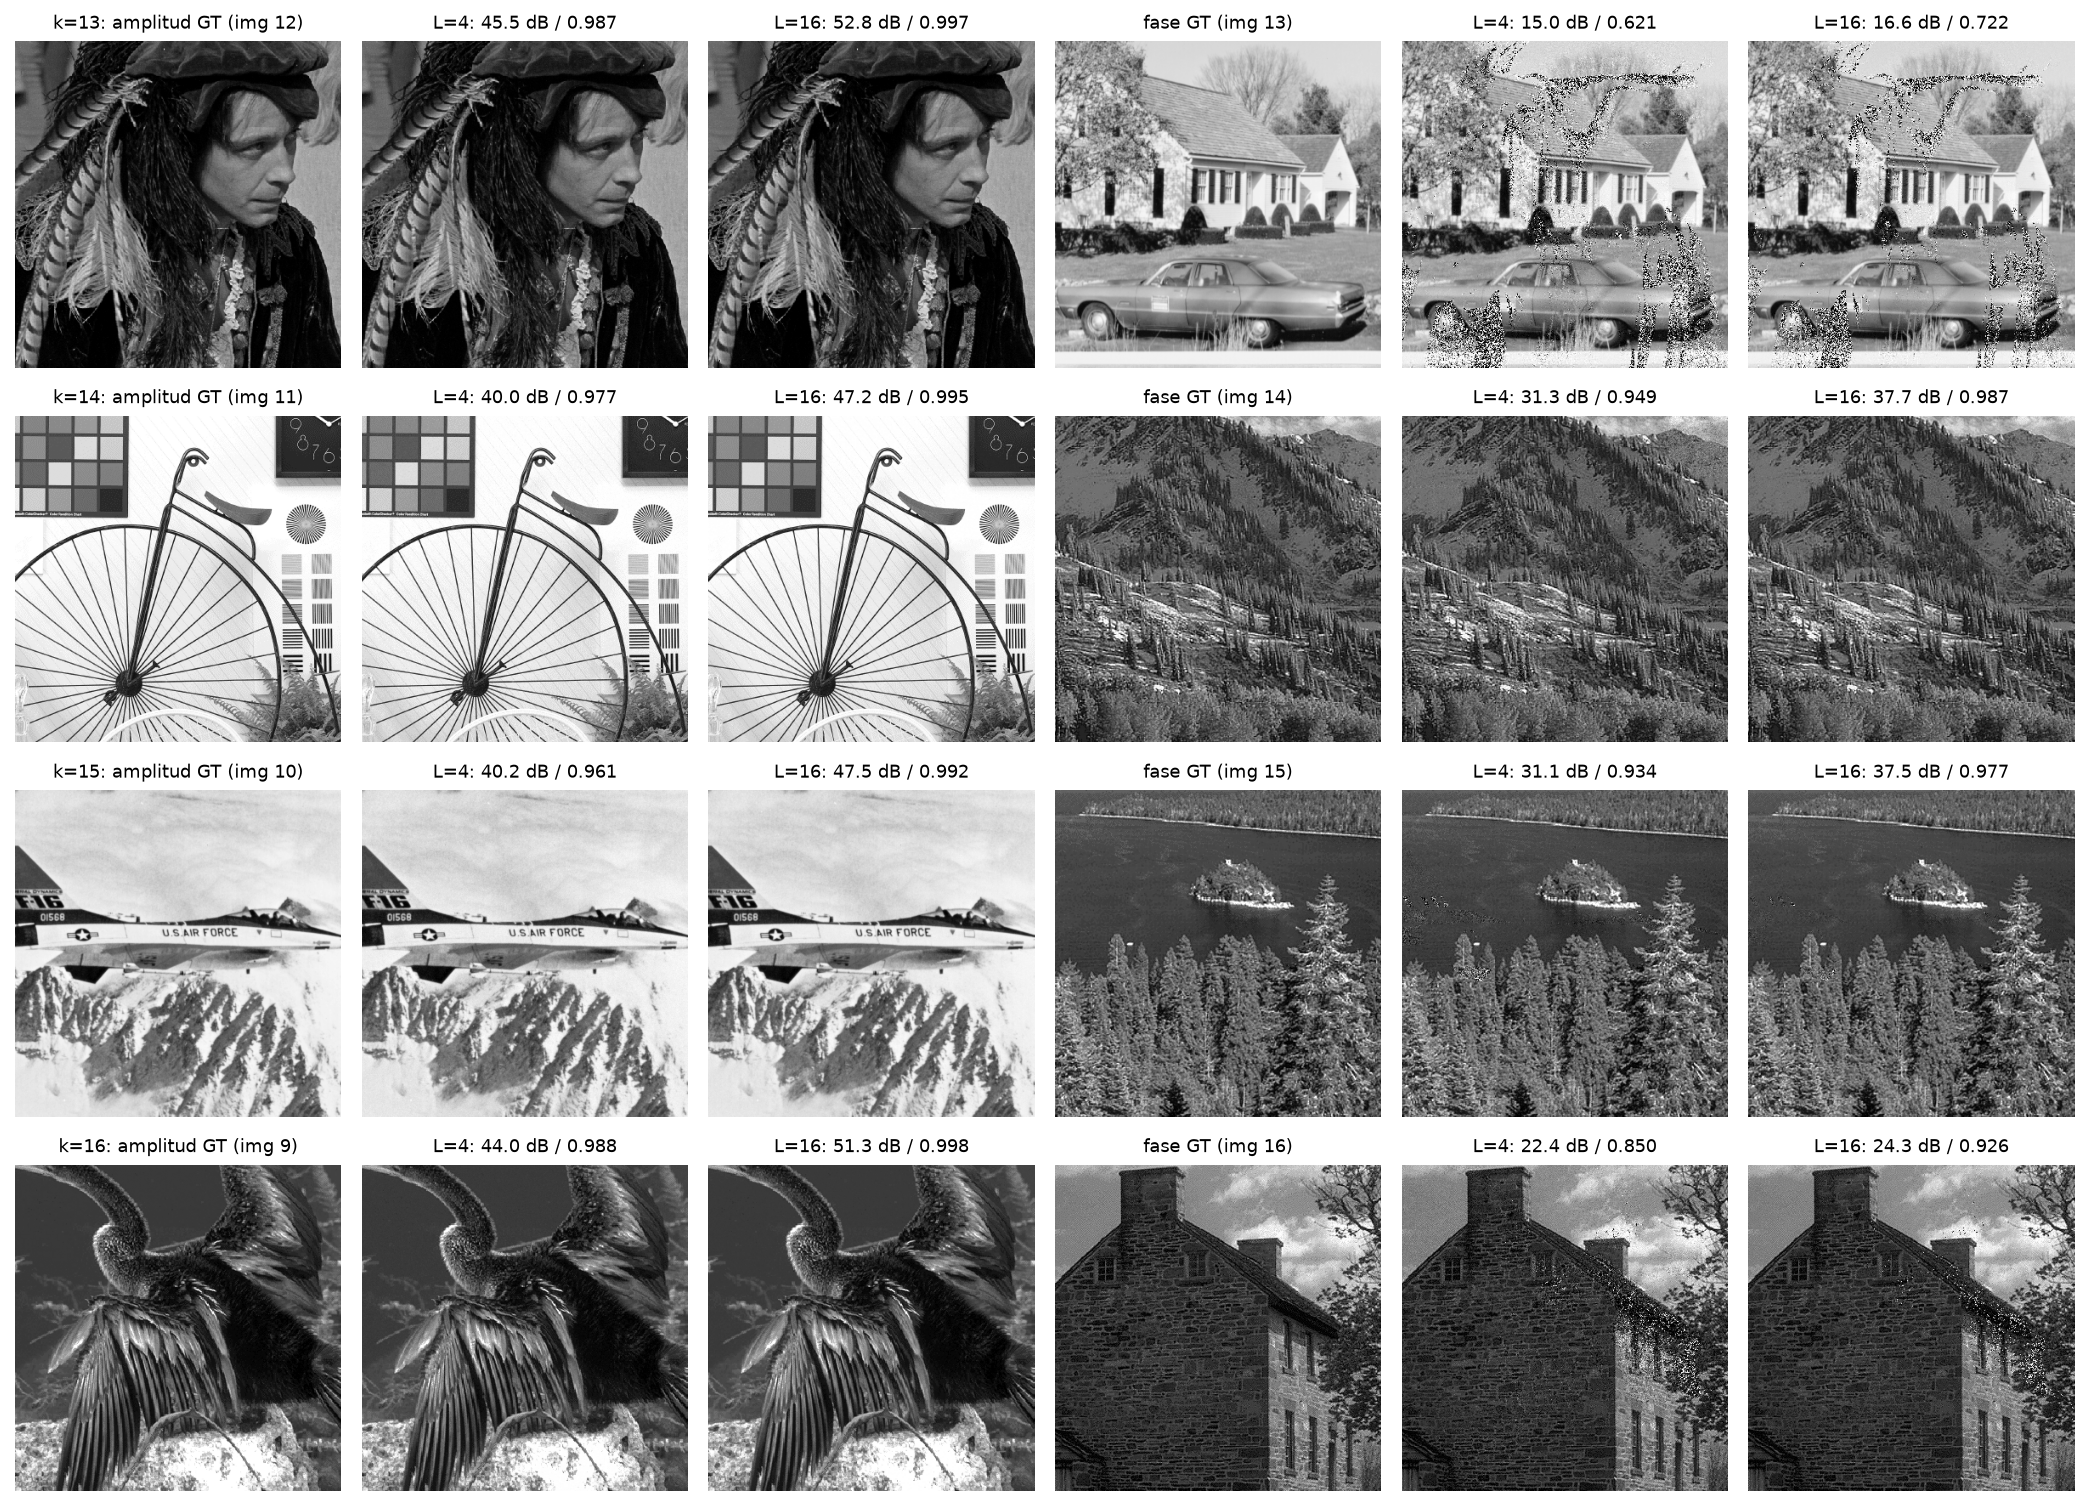
\includegraphics[height=0.78\textheight,keepaspectratio]{Fig/anexo_comparaciones_13_16.png}
    \caption{Reconstrucciones de los objetos 13--16.}
    \label{fig:anexo-13-16}
\end{figure}

\clearpage
\begin{figure}[H]
    \centering
    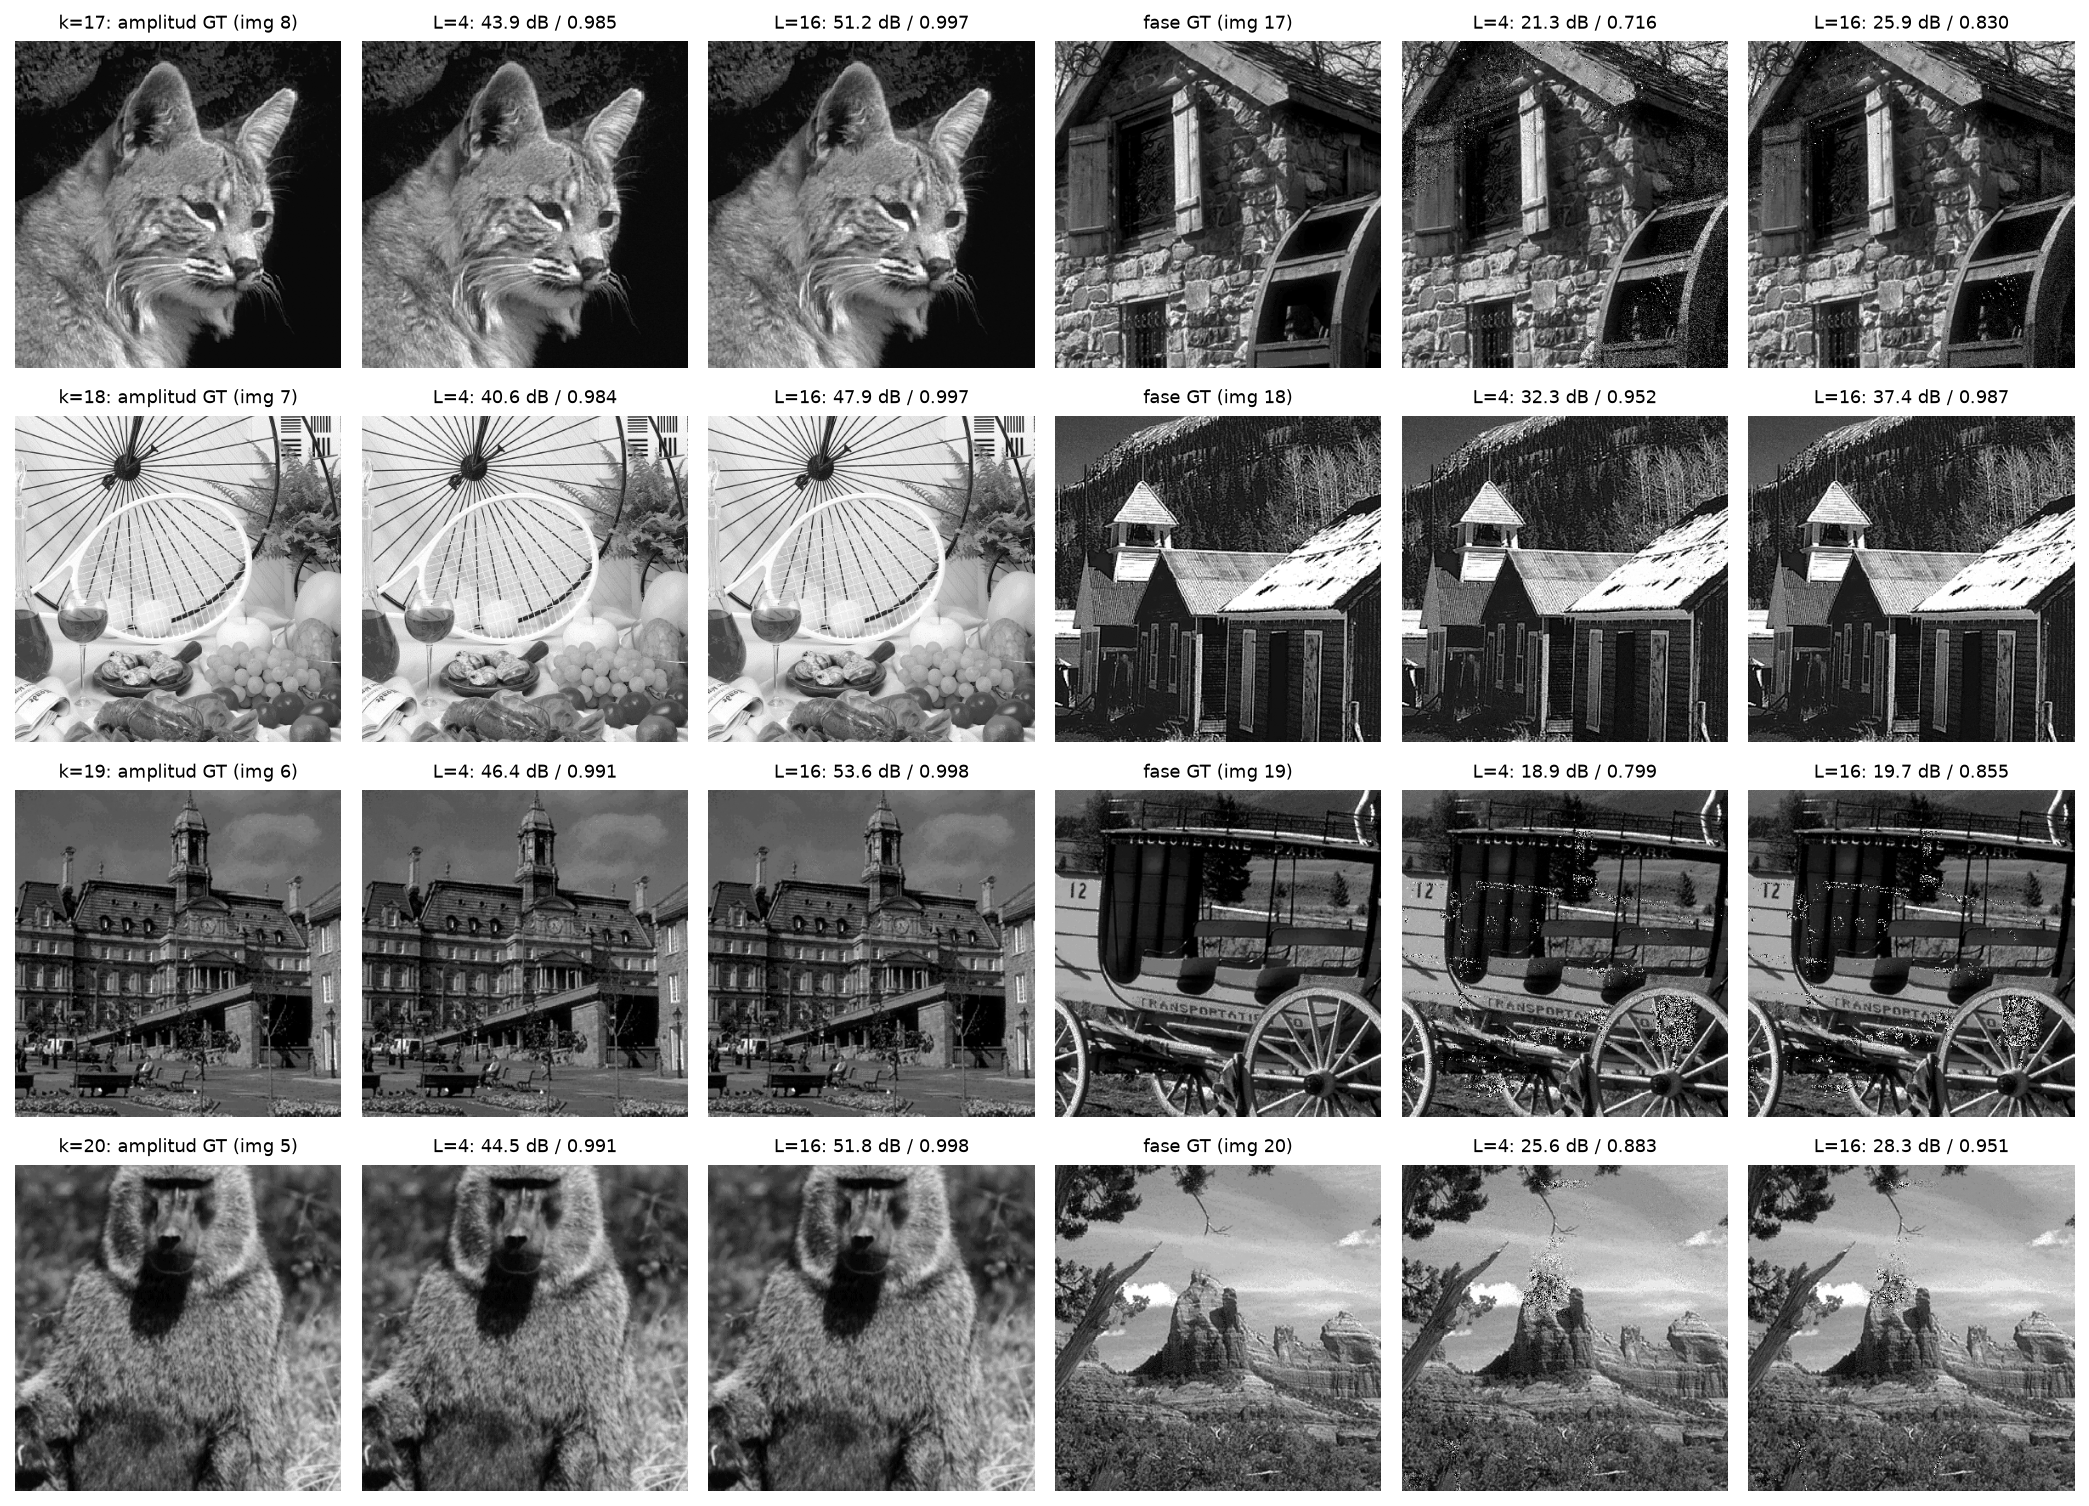
\includegraphics[height=0.78\textheight,keepaspectratio]{Fig/anexo_comparaciones_17_20.png}
    \caption{Reconstrucciones de los objetos 17--20.}
    \label{fig:anexo-17-20}
\end{figure}

\clearpage
\begin{figure}[H]
    \centering
    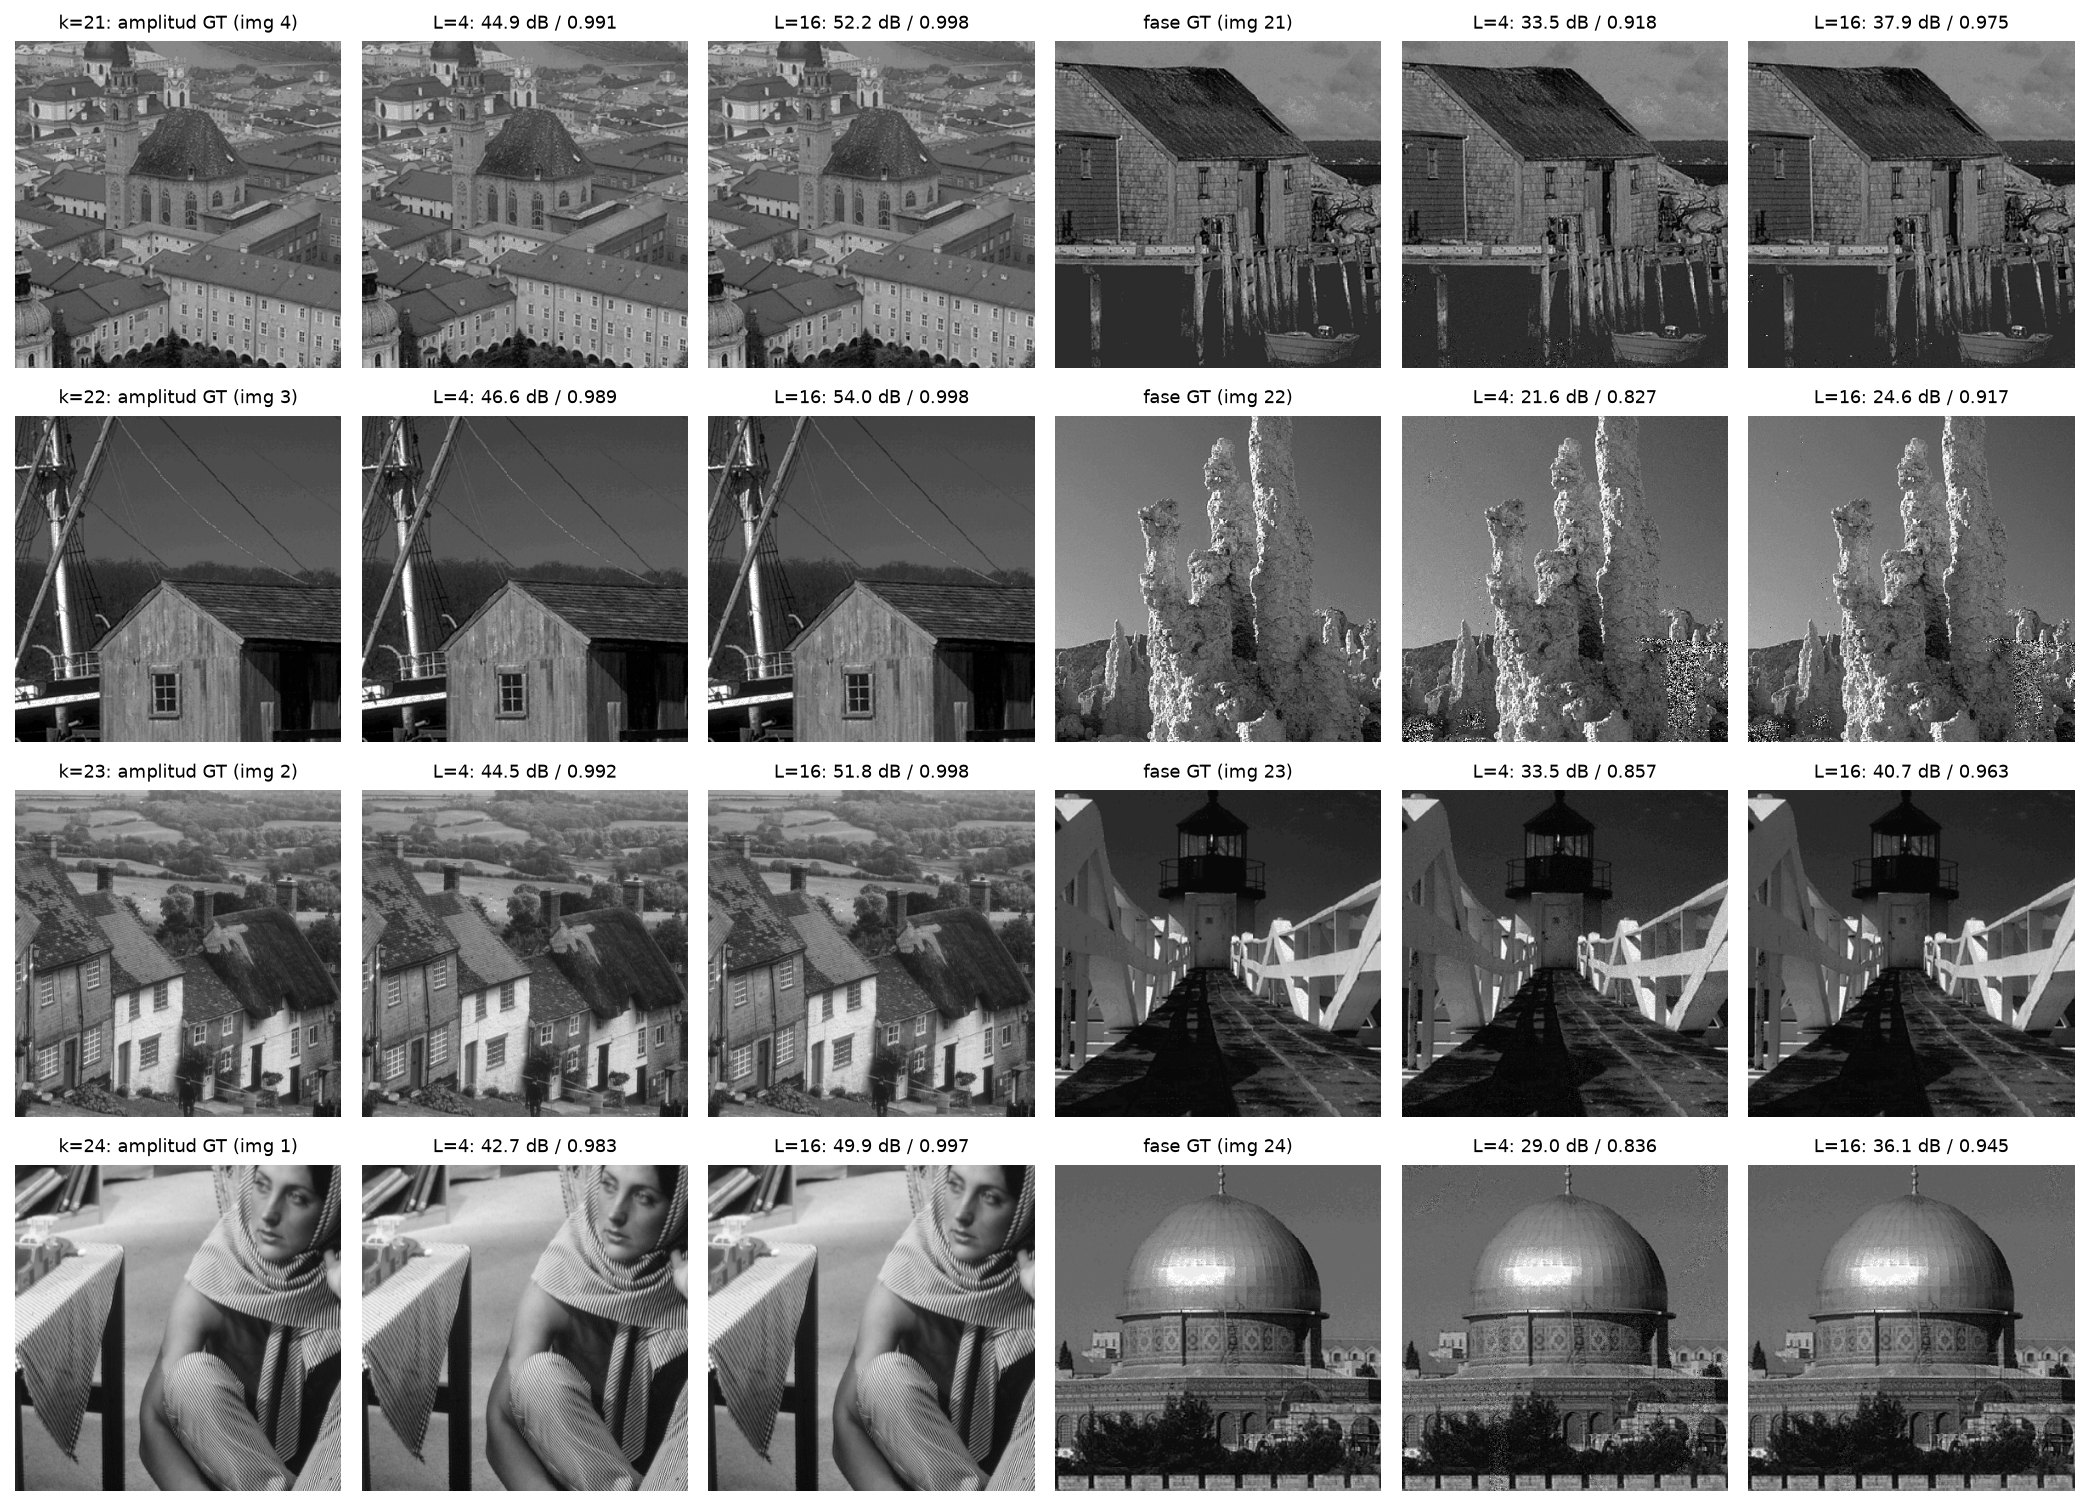
\includegraphics[height=0.78\textheight,keepaspectratio]{Fig/anexo_comparaciones_21_24.png}
    \caption{Reconstrucciones de los objetos 21--24.}
    \label{fig:anexo-21-24}
\end{figure}
\end{landscape}

\end{document}
